\chapter{Learning data from a resolved liquid jet in crossflow}
	\label{ch5:jicf_resolved_simulations}



Describe here all our simulations done with JICF, what we have achieved with them, etc.

\begin{itemize}

	\item Experimental setup description
	
	\item Numerical setup description. Operating points
	
	\item Mesh convergence study
	
	\item Spray sampling
	
	\item Direct measurement of fluxes with interior boundaries
	
	\item Liquid disappearing (set levelset band ) ??
	
	\item Results:
	
		\begin{itemize}
		
			\item Breakup mechanisms
			
			\item In-nozzle phenomena of flow separation (and entrainment of gaseous bubbles)
			
			\item Spray formation and evolution with axial distance
	
		\end{itemize}
		
	\item Other results:
	
		\begin{itemize}
		
			\item Slip velocity evolution
			
			\item Vorticity distribution (horse-shoe vortices, double vortical structural in liquid)
		
		\end{itemize}

\end{itemize}

\newpage 

\section{Introduction}

The previous chapter has detailed the theory of the proposed models to build lagrangian injectors for initialising dispersed phase simulations, named Smart Lagrangian Injectors (SLI). These models, nowadays in its earliest state of maturity, are intended to be generic and applicable to a broad range of operating conditions and injector configurations. To show its capabilities, they have been developed in their first stage with resolved simulations of liquid jet in crossflow (JICF) configuration. This chapter details these simulations, performed with the software YALES2 \citepColor[moureau_design_2011]. % \textbf{https://reader.elsevier.com/reader/sd/pii/S1631072110002111?token=9137B6903478D4E8E427F5D8218DFC3EB42446DB034970B14BA9DE87AA7E80D130124A7EF8D8608D21D5D465CCE05A4F&originRegion=eu-west-1&originCreation=20210524114835}

The fundamentals and the physics of non-reactive JICF have been introduced in $\S$\ref{sec:ch1_fuel_injection_technology}. This chapter shows the results, analysis and injectors obtained from a kerosene JICF simulation replicating the experimental facility tested by \citeColor[becker_breakup_2002]. This configuration is used for validating the models. Section \ref{sec:ch5_experimental_bench} displays the experimental test bench, whose numerical setup and operating conditions chosen for numerical computations are detailed in Section \ref{sec:computational_setup}.


\section{Experimental test case}
	\label{sec:ch5_experimental_bench}

The experimental configuration tested by \citeColor[becker_breakup_2002] is shown in Figure \ref{fig:experiment_JICF_DLR}. The test rig is shown at the left. Liquid kerosene is injected through the atomizer ports to a quartz glass duct of rectangular cross section $25$x$40$ mm$^2$. The duct inlet is located at $120$ mm upstream the injection port. The boundary layer thickness developing along the bottom of the duct has been measured experimentally just upstream the atomizer, being between $4$ and $5$ mm. The lateral walls allow for optical access from the atomizer port until a location at 100 mm downstream. Air is introduced through two separate channels, a main one and a supplementary one. The main airflow is injected at the inlet of the quartz duct, while the supplementary one passes around it. Both airflows merge at the end of the duct and leave the domain through a common exit acting as a sonic throttle. The velocity inside the quartz can then be tuned by varying the size of the nozzle and the supplementary air flow rate. In the experiments performed, the range of air velocities goes from $u_g = 50$ to 100 m/s and the range of pressure from $p$ = 1.5 to 15 bar, hence allowing the study high-pressure conditions. The air temperature is maintained to $T_g = 290$ K. The fuel tested was kerosene Jet A-1 with density $\rho_l = 795$ kg m$^{-3}$ and surface tension $\sigma = 22 \cdot 10^{-3}$ N m$^{-1}$.

The liquid injection nozzle can be seen in Figure \ref{fig:experiment_JICF_DLR} right. It consists of a plain jet nozzle of $d_\mathrm{inj} =  0.45$ mm diameter and $L/d_\mathrm{inj}$ ratio of 1.56 with sharp edges. The average discharge coefficient for the mass flow rates of interest in the experimental studies is $0.6$. More details on the test rig can be found in \citeColor[brandt_experimental_1997].

\begin{figure}[h!]
	\centering
	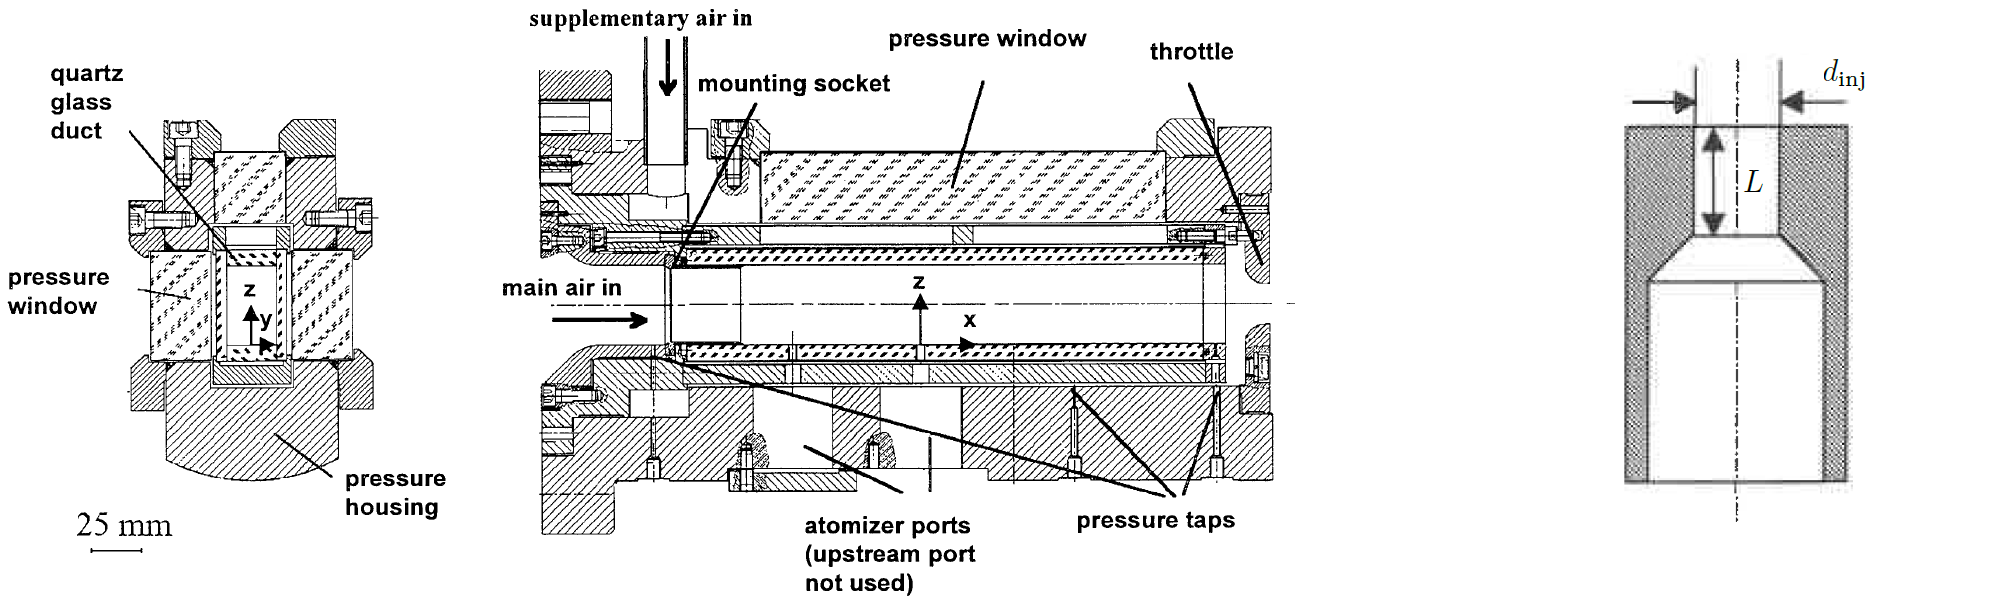
\includegraphics[scale=0.35]{./part2_developments/figures_ch5_resolved_JICF/experiment_JICF_DLR}
	\caption[JICF experimental setup]{JICF experimental setup. \textsl{Left}: Test rig. \textsl{Right}: liquid nozzle geometry employed in the experimental study. Source: \citeColor[becker_breakup_2002]}
	\label{fig:experiment_JICF_DLR}
\end{figure}


A correlation for the trajectory of the jet was obtained experimentally by analysing optically its penetration for the several operating conditions tested. It corresponds to the trajectory of the jet's windward side, and gives a relation between the vertical location $z$ with respect to the axial coordinate $z$ as a function of the nozzle diameter $d_\mathrm{inj}$ and the momentum ratio $q$ defined by Eq. (\ref{eq:q_and_We_JICF_parameters}): % The rorrelation has a standard deviation of 0.81.

\begin{equation}
    \label{eq:jicf_trajectory_becker}
    \frac{z}{d_\mathrm{inj}} = 1.57 \mathrm{q}^{0.36} \ln \left( 1 + 3.81 \frac{x}{d_\mathrm{inj}} \right)
\end{equation}



\section{Computational setup}
	\label{sec:computational_setup}

%\subsection*{Numerical domain and baseline mesh}

Figure \ref{fig:numerical_setup_maquette_JICF_DLR} shows the computational domain developed to replicate the simulations of the test bench shown in Figure \ref{fig:experiment_JICF_DLR}. The duct is modelled as a plenum consisting of a box of dimensions 25x40x270 mm$^3$. The hydraulic diameter of the duct cross section, which is used to calculate the gas Reynolds number, is $D_h = 30.8$ mm. A magnified view of the nozzle is also shown, with diameter $0.45$ mm and straight section length of 0.7 mm prior to injection to keep $L/D = 1.56$ as in the experiments. The boundary conditions are also indicated. The plenum walls use a wall law of logarithmic type except closer to the domain pressure outlet, which have been set to slip walls to avoid backflow. The nozzle walls are rigid walls. For the liquid inlet, a Poiseuille profile has been specified, while in the gaseous inlet a mean velocity profile has been set in order to recover the boundary layer thickness of between 4 and 5 mm upstream the injection nozzle as described in the experiments (see Appendix \ref{app:JICF_BL_setup} for details). Due to the high Reynolds number at the gaseous inlet (see Table \ref{tab:jicf_operating_conditions}), synthetic turbulence is added in the liquid inlet (details given in $\S$\ref{sec:ch5_initial_conditions}).

\begin{figure}[ht]
     \centering
     \includeinkscape[scale=0.35]{./part2_developments/figures_ch5_resolved_JICF/DLR_becker_numerical_config}
      \caption{Numerical domain and boundary conditions of the experimental test bench of \citeColor[becker_breakup_2002]. \textsl{Left}: complete domain. \textsl{Right}: detailed view of the injection nozzle. All dimensions are in mm.}
      \label{fig:numerical_setup_maquette_JICF_DLR}
\end{figure}

Figure \ref{fig:jicf_dlr_mesh} shows the baseline mesh, where the symmetry plane at $y = 0$ is displayed. It is composed of 66 million tetrahedral cells. The baseline cell size in the channel upstream liquid injection is 0.5 mm, while the cells located in the downstream region have an average size of 3 mm. The element size at the near-field region is 0.7 mm, and within the discharge section of the liquid nozzle it is refined to to $20 \mu m$. The justification of this mesh is done at $\S$\ref{sec:ch5_initial_conditions}, where a mesh independence study of the gaseous field is carried out. This mesh is used at the beginning of all the simulations performed, but then it change dynamically in each simulation as more liquid is introduced in the domain due to the AMR routine that refines the mesh at the liquid-gas interface ($\S$\ref{sec:YALES2}). Simulations are performed with the ACLS methodology describe in $\S$\ref{subsec:ch2_ACLS}.

\begin{figure}[h!]
	\centering
	\includeinkscape[inkscapelatex=false,scale=0.7]{./part2_developments/figures_ch5_resolved_JICF/jicf_mesh/jicf_mesh}
	\caption[Baseline JICF mesh, showing magnified views of the near-field and nozzle regions.]{Baseline JICF mesh, showing magnified views of the near-field and nozzle regions. The red rectangle is the region where meshes are shown in the mesh convergence study of $\S$\ref{sec:ch5_initial_conditions}}
	\label{fig:jicf_dlr_mesh}
\end{figure}



\section{Operating conditions}

Two operating conditions tested experimentally in \citeColor[becker_breakup_2002] have been simulated. Both of them have the same momentum ration $q = 6$ but differ in the Weber number: $We_g = 830$ (low Weber) and $We_g = 1470$ (low Weber). According to the values of $q$ and $We_g$, the former condition corresponds to surface breakup dominating regime while the latter is located at the dividing line between column and surface breakup. Figure \ref{fig:location_JICF_ops_in_breakup_map} shows the location of both operating points in the breakup map of \citeColor[wu_breakup_1997]. The physical magnitudes and dimensionless numbers of both operating points are shown in Table \ref{tab:jicf_operating_conditions}. Apart from the values $q$ and $We_g$, the dimensionless numbers in  Eq. (\ref{eq:dimensionless_numbers_jicf}) are also calculated: the liquid and gaseous Reynolds numbers $Re_g$ and $Re_g$ respectively, Ohnesorge number $Oh$, aerodynamic Weber $We_\mathrm{aero}$, relative Weber $We_\mathrm{rel}$ and density ratio $r$. These numbers have been added since they are defined in several experimental studies \citeColor[wu_breakup_1997,becker_breakup_2002,ragucci_trajectory_2007] to characterize the operating points tested. 

For performing the computations of resolved atomization, the ACLS methodology combined with the AMR routine described in $\S$\ref{subsec:ch2_ACLS} is used. For each simulation, two interface mesh sizes have been simulated: $\Delta x_\mathrm{min} = 20 ~\mu m$ (coarse case) and $\Delta x_\mathrm{min} = 10 ~\mu m$ (fine case). Therefore, a total of four simulations have been done. The nomenclature for each simulation, which is used hereafter in this document, is introduced in Table \ref{tab:jicf_resolved_simulations_performed}.

%\begin{subequations}
%\label{eq:dimensionless_numbers_jicf}
%\begin{align}
%Re_l &= \frac{\rho_l u_l d_\mathrm{inj}}{\mu_l}\\
%Re_g &= \frac{\rho_g u_g D_h}{\mu_g}\\
%We_\mathrm{aero} &= \frac{\rho_g u_l^2 d_\mathrm{inj}}{\sigma}  \\
%We_\mathrm{rel} &= \frac{\rho_g \left( u_g - u_l \right)^2 d_\mathrm{inj}}{\sigma} \\
%Oh &=  \frac{\mu_l}{\sqrt{\rho_l \sigma d_\mathrm{inj}}}\\
%r &= \frac{\rho_l}{\rho_g} 
%\end{align}
%\end{subequations}

%\begin{align}
%\label{eq:dimensionless_numbers_jicf}
%Re_l &= \frac{\rho_l u_l d_\mathrm{inj}}{\mu_l}          &  Re_g &= \frac{\rho_g u_g D_h}{\mu_g}              &  Oh &=  \frac{\mu_l}{\sqrt{\rho_l \sigma d_\mathrm{inj}}}\\
%We_\mathrm{aero} &= \frac{\rho_g u_l^2 d_\mathrm{inj}}{\sigma}    &  We_\mathrm{rel} &= \frac{\rho_g \left( u_g - u_l \right)^2 d_\mathrm{inj}}{\sigma}          & r &= \frac{\rho_l}{\rho_g} 
%\end{align}


\begin{equation}
\label{eq:dimensionless_numbers_jicf}
\begin{aligned}
Re_l &= \frac{\rho_l u_l d_\mathrm{inj}}{\mu_l}          &  Re_g &= \frac{\rho_g u_g D_h}{\mu_g}              &  Oh &=  \frac{\mu_l}{\sqrt{\rho_l \sigma d_\mathrm{inj}}}\\
We_\mathrm{aero} &= \frac{\rho_g u_l^2 d_\mathrm{inj}}{\sigma}    &  We_\mathrm{rel} &= \frac{\rho_g \left( u_g - u_l \right)^2 d_\mathrm{inj}}{\sigma}          & r &= \frac{\rho_l}{\rho_g} 
\end{aligned}
\end{equation}

\begin{table}[!h]
\centering
\caption{JICF operating points studied}
\begin{tabular}{lcccc}
\thickhline
\textbf{Parameter} & \textbf{Symbol} & \textbf{Units} &  \textbf{Low Weber} &  \textbf{High Weber} \\ %\textbf{WE\_880} &  \textbf{WE\_1470} \\
\thickhline
Nozzle diameter & $d_\mathrm{inj}$ & mm & 0.45 & 0.45 \\
%\hline
Gas bulk velocity & $u_g$ & m s$^{-1}$ & 75 & 100 \\
%\hline
Gas flow rate & $Q_g$ & m$^3$ s$^{-1}$ & 0.075  & 0.1 \\
%\hline
Liquid bulk velocity & $u_l$ & m s$^{-1}$ & 17.5  & 23.33 \\
%\hline
Liquid flow rate & $Q_l$ & mm$^3$ s$^{-1}$ & 2783  & 3710 \\
%\hline
Ambient pressure & $p_\mathrm{amb}$ & bar &  6 & 6 \\
%\hline
Gas temperature & $T_g$ & K & 290 & 290 \\
%\hline
Liquid temperature & $T_l$ & K & 288 & 288 \\
%\hline
Gas density & $\rho_g$ & kg m$^{-3}$ &  7.21 & 7.21 \\
%\hline
Liquid density & $\rho_l$ & kg m$^{-3}$ &  795 & 795  \\
%\hline
Gas viscosity & $\mu_g$ & kg m$^{-1}$ s$^{-1}$ & $1.8162 \cdot 10^{-5}$ &  $1.8162 \cdot 10^{-5}$  \\
%\hline
Liquid viscosity & $\mu_l$ & kg m$^{-1}$ s$^{-1}$ & $1.5 \cdot 10^{-3}$ & $1.5 \cdot 10^{-3}$  \\
%\hline
Surface tension & $\sigma$ & kg s$^{-2}$ &  0.022 & 0.022  \\
\thickhline
Momentum ratio & $q$ & - & 6 & 6 \\
%\hline
Gas Reynolds number & $Re_g$ & - & $0.92 \cdot 10^6$ & $1.22 \cdot 10^6$ \\
%\hline
Liquid Reynolds number & $Re_l$ & - & 4170 & 5560 \\
%\hline
Gas Weber number & $We_g$ & - & 830 & 1470 \\
%\hline
Liquid Weber number & $We_l$ & - & 5000 & 8850 \\
%\hline
Relative Weber number & $We_\mathrm{rel}$ & - & 490 & 870 \\
%\hline
Aerodynamic Weber number & $We_\mathrm{aero}$ & - & 45 & 80 \\
%\hline
Ohnesorge number & $Oh $ & - & 0.017 & 0.017 \\
%\hline
Density ratio & $r$ & - & 110 & 110 \\
%\hline
%Viscosity ratio & $\mu_l/\mu_g$ & [-] &  \multicolumn{2}{|c|}{1} \\
\thickhline
\end{tabular}
\label{tab:jicf_operating_conditions}
\end{table}

\clearpage


\begin{table}[!h]
\centering
\caption{Nomenclature for resolved atomization simulations}
\begin{tabular}{ccc}
\thickhline
%$\pmb{\Delta} x_\mathrm{min}$ [$\pmb{\mu}$$\textbf{m}])  &  \multicolumn{2}{c}{\textbf{Operating condition}} \\ 
$\Delta x_\mathrm{min}$ [$\mu$m]  &  \multicolumn{2}{c}{\textbf{Operating condition}} \\ 
\cline{2-3}
 &  Low $We_g$ &  High $We_g$ \\ 
\thickhline
\textbf{10} & UG75\_DX10 & UG100\_DX10 \\
\textbf{20} & UG75\_DX20 & UG100\_DX20 \\
\thickhline
\end{tabular}
\label{tab:jicf_resolved_simulations_performed}
\end{table}

\begin{figure}[ht]
     \centering
     \includeinkscape[inkscapelatex=false,scale=0.6]{./part2_developments/figures_ch5_resolved_JICF/jicf_breakup_regime_our_operating_points}
     \caption{Location of simulated operating conditions in the breakup map by \citeColor[wu_breakup_1997]}
	% See: https://stackoverflow.com/questions/35210337/can-i-plot-several-histograms-in-3d/35225919
      \label{fig:location_JICF_ops_in_breakup_map}
\end{figure}



%\section{YALES2 code (??)}

\section{Tools and methodologies}

%\subsection{Spray sampling in resolved simulations}

\subsection{Numerical computation of jet trajectory}
	\label{sec:ch5_tools_jicf_trajectories}

One of the most important characteristics of a jet in crossflow is its trajectory (see $\S$\ref{sec:ch1_fuel_injection_technology}). This feature determines how far the jet penetrates in the domain and has a paramount effect on the latter evaporation and mixing processes, hence affecting the flame dynamics. Experimental studies often provide correlations for the trajectory of the windward side of the jet (see Table \ref{tab:correlations_experimental_JICF}), such as the one from Eq. (\ref{eq:jicf_trajectory_becker}). These correlations depend generally on the momentum flux ratio $q$, the injection diameter $d_\mathrm{inj}$ and, in some case \citepColor[ragucci_trajectory_2007], in the Weber number $We$. The overall dependency of the trajectory on these parameters is still unknown.

Experimentally, researches have used different approaches to obtain trajectories based on the different optical techniques employed. Many works \citemColor[becker_breakup_2002,stenzler_penetration_2003,freitag_spray_2008] obtain instantaneous images of the jet with shadowgraphy techniques and then MIE scattering or emboss-filter operations to obtain binary images where liquid and gas phases can be clearly distinguished. Then, images are averaged and the vertical penetration is obtained by detecting the coordinates where the light intensity gradients are maximum. The image averaging can be performed before or after the filtering operations. These methods, which are based on obtaining the trajectories from mean images, are hereafter denoted as \textbf{mean trajectory methods}. Figure \ref{fig:expe_obtention_of_trajectories} shows an illustration of such experimental methodology from the work by \citeColor[stenzler_penetration_2003]. The filtering operations and way to obtain the light gradients vary among authors. Other works \citepColor[ragucci_trajectory_2007] use the same principles of filtering and binarization, but obtain the trajectories from instantaneous jet images. Then, the instantaneous trajectories are averaged to yield the mean trajectories. These methods are hereafter denoted as \textbf{instantaneous trajectory methods}.

From a computational perspective, similar methodologies can be applied to obtain the jet trajectories from simulations. The same sequence of operations as shown in Figure \ref{fig:expe_obtention_of_trajectories} used to process experimental images could be applied to numerical snapshots of the JICF. Nevertheless, the ACLS methodology presents the advantage that the interface can be clearly defined with the $\psi$ function, and hence it can be used to obtain the trajectory by different methods. In this work, four methodologies to obtain the numerical trajectories from JICF resolved simulations are presented. As in the experimental classification previously suggested to obtain trajectories, these methodologies are also distinguished as \textbf{mean trajectory methods} or \textbf{instantaneous trajectory methods}, depending on whether they use the mean or instantaneous $\psi$ field respectively. Two methods for each category are detailed in this section, while the results obtained are shown in $\S$\ref{subsec:ch5_jet_trajectories_results}.

\begin{figure}[ht]
     \centering
     \includeinkscape[inkscapelatex=false,scale=0.6]{./part2_developments/figures_ch5_resolved_JICF/trajectories_obtention/expe_obtention}
     \caption{Illustration of experimental procedure to obtain trajectories. Figures taken from \citeColor[stenzler_penetration_2003]}
      \label{fig:expe_obtention_of_trajectories}
\end{figure}


\subsubsection{Instantaneous trajectory methods}

The averaged numerical trajectories can be obtained from instantaneous solutions of the jet by obtaining the instantaneous trajectories for every solution obtained and then averaging them. Figure \ref{fig:trajectory_obtention_instantaneous_general} shows the procedure to extract the interface contour that is later used to obtain the trajectories. First, the liquid-gas interface is plotted in the domain as a surface of iso-contour $\Gamma: \psi = 0.5$ (Figure \ref{fig:trajectory_obtention_instantaneous_general} left), and then this contour is extracted at the central plane $y = 0$, as indicated by the black line of Figure \ref{fig:trajectory_obtention_instantaneous_general} right. 

\begin{figure}[ht]
     \centering
     \begin{subfigure}[b]{0.45\textwidth}
         \centering
         \includeinkscape[inkscapelatex=false,scale=0.35]{./part2_developments/figures_ch5_resolved_JICF/trajectories_obtention/instantaneous_interface_3D}
         %\caption{Instantaneous jet interface}
     \end{subfigure}
     %\hfill
     \begin{subfigure}[b]{0.45\textwidth}
         \centering
         \includeinkscape[inkscapelatex=false,scale=0.35]{./part2_developments/figures_ch5_resolved_JICF/trajectories_obtention/instantaneous_interface_y0}
         %\caption{Contour of instantaneous interface at plane y = 0}
     \end{subfigure}
        \caption[Procedure to obtain instantaneous trajectories.]{Procedure to obtain instantaneous trajectories. \textsl{Left}: instantaneous jet interface. \textsl{Right}: contour of instantaneous interface at plane y = 0}
	% See: https://stackoverflow.com/questions/35210337/can-i-plot-several-histograms-in-3d/35225919
        \label{fig:trajectory_obtention_instantaneous_general}
\end{figure}

Once the interface is obtained at $y = 0$, the outer contour of the trajectory must be obtained. This is the one corresponding to the windward side of the jet, and hence the one defining the instantaneous trajectory. For its obtention, the $z$ axis is swept and the points belonging to the trajectory are obtained as follows:

\begin{enumerate}

	\item The $z$ axis is discretized in intervals with thickness $\Delta z$. 
	
	\item For each interval, the contour point with minimum $x$ coordinate is obtained.
	
	\item Points are sorted according to their $x$ coordinate, defining the trajectory.

\end{enumerate}

This procedure is repeated at every instantaneous snapshot of the jet to obtain the instantaneous trajectories. Then, all the trajectories obtained are interpolated to obtain the mean trajectories which can be compared to experimental correlations. This method is similar to the experimental methodology employed by \citeColor[ragucci_trajectory_2007] to obtain mean trajectories, and was used by \citeColor[leparoux_primary_2018] to simulate their experimental configuration and compare numerical trajectories with experiments. However, it differs from the methodology employed by \citeColor[becker_breakup_2002], whose experimental test rig is simulated in this work and who obtain the trajectories with a methodology more similar to the mean trajectory methods (see next point). Still, it is worth to investigate the instantaneous methodologies to obtain the trajectories and to compare them with the mean methods.

The procedure previously described works properly in the dense core, where the interface contour is continuous up to the breakup point $z_b$. After this location, atomization takes place and the detected $\Gamma$ contours belong to ligaments or droplets. In this case, the definition of \textsl{outer trajectory} does not hold as clearly as in the dense core: some contours detected might belong to satellite droplets or to drops originated from surface breakup, and could modify the final average trajectory by lowering it down. With this consideration, two different trajectories are distinguished in the instantaneous methodologies: \textbf{non-monotonic} and \textbf{monotonic} trajectories. These are discussed in the following lines.

%\subsubsection*{Non-monotonic trajectory}

\paragraph*{{Non-monotonic trajectory}} 

Non-monotonic instantaneous trajectories can be obtained by applying the methodology as explained in the previous lines, accounting also for the contours which a priori do not pertain to the outer contour of the instantaneous trajectory. This procedure is illustrated in Figure \ref{fig:trajectory_obtention_instantaneous_method_a}: the different points of the trajectory are obtained when sweeping the $z$ axis, and the instantaneous trajectory is obtained by joining these points. Then, sorting all the sampled points along the $x$ axis creates a non-monotonic trajectory since some contour points belong to liquid structures further downstream, see Figure \ref{fig:trajectory_obtention_instantaneous_method_a} right.

\begin{figure}[ht]
     \centering
     \begin{subfigure}[b]{0.45\textwidth}
         \centering
         \includeinkscape[inkscapelatex=false,scale=0.35]{./part2_developments/figures_ch5_resolved_JICF/trajectories_obtention/method_a_sweep_nonMonotonic}
         %\caption{Instantaneous jet interface}
     \end{subfigure}
     %\hfill
     \begin{subfigure}[b]{0.45\textwidth}
         \centering
         \includeinkscape[inkscapelatex=false,scale=0.34]{./part2_developments/figures_ch5_resolved_JICF/trajectories_obtention/method_a_inst_trajectory}
         %\caption{Contour of instantaneous interface at plane y = 0}
     \end{subfigure}
        \caption[Obtention of non-monotonic instantaneous trajectory]{Obtention of non-monotonic instantaneous trajectory. \textsl{Left}: sweep process along z axis of interface points. \textsl{Right}: instantaneous trajectory.}
	% See: https://stackoverflow.com/questions/35210337/can-i-plot-several-histograms-in-3d/35225919
        \label{fig:trajectory_obtention_instantaneous_method_a}
\end{figure}

\clearpage

%\subsubsection*{Monotonic trajectory}
\paragraph*{Monotonic trajectory} 

The procedure is identical to the obtention of non-monotonic trajectories with one fundamental difference: when sorting along the $x$ axis, only points with increasing $z$ coordinate are considered. In this way, a monotonic trajectory is obtained, see Figure \ref{fig:trajectory_obtention_instantaneous_method_b} right. 


\begin{figure}[ht]
     \centering
     \begin{subfigure}[b]{0.45\textwidth}
         \centering
         \includeinkscape[inkscapelatex=false,scale=0.35]{./part2_developments/figures_ch5_resolved_JICF/trajectories_obtention/method_b_sweep_monotonic}
         %\caption{Instantaneous jet interface}
     \end{subfigure}
     %\hfill
     \begin{subfigure}[b]{0.45\textwidth}
         \centering
         \includeinkscape[inkscapelatex=false,scale=0.33]{./part2_developments/figures_ch5_resolved_JICF/trajectories_obtention/method_b_inst_trajectory}
         %\caption{Contour of instantaneous interface at plane y = 0}
     \end{subfigure}
        \caption[Obtention of monotonic instantaneous trajectory]{Obtention of monotonic instantaneous trajectory. \textsl{Left}: sweep process along z axis of interface points, excluding points whose vertical location is lower than the vertical location of the previous ones. \textsl{Right}: instantaneous trajectory.}
	% See: https://stackoverflow.com/questions/35210337/can-i-plot-several-histograms-in-3d/35225919
        \label{fig:trajectory_obtention_instantaneous_method_b}
\end{figure}

The two instantaneous methodologies described here will provide the same trajectories in the dense core, but will differ after the breakup point. Therefore, the trajectories obtained from this methodology can be compared and used to estimate an average position of the dense core. 


\subsubsection{Mean trajectory methods}

Another possibility to obtain mean trajectories is by using the mean field of the levelset function, $\overline{\psi}$. An example of a converged $\overline{\psi}$ field is shown in Figure \ref{fig:trajectory_obtention_mean_methods_c_d} left.. This requires the accumulation of statistics over a certain time (instantaneous trajectories do not need accumulation statistics as long as the instantaneous $\psi$ field is available), but presents the advantage that the jet trajectory can be obtained with one single $\overline{\psi}$ field once convergence is achieved. In this category, two different methods are used: the \textbf{maximum gradient method} and the \textbf{iso-contour method}.

\begin{figure}[ht]
     \centering
     \includeinkscape[inkscapelatex=false,scale=0.35]{./part2_developments/figures_ch5_resolved_JICF/trajectories_obtention/methods_c_d_and_mean_psi_field}
     \caption[Methods based on mean trajectories]{Methods based on mean trajectories. \textsl{Left}: $\overline{\psi}$ field. \textbf{Center}: $\max \left( \nabla_z | \overline{\psi} | \right)$ contour. \textsl{Right}: contour $\overline{\psi} = 0.01$.}
	% See: https://stackoverflow.com/questions/35210337/can-i-plot-several-histograms-in-3d/35225919
      \label{fig:trajectory_obtention_mean_methods_c_d}
\end{figure}



\paragraph{Maximum gradient method}

This method is more similar to the experimental methods presented in \citeColor[becker_breakup_2002], \citeColor[stenzler_penetration_2003] and \citeColor[freitag_spray_2008]. In these works, the jet trajectory is obtained as the contour of the maximum intensity gradient in the vertical direction of the mean jet (see Figure \ref{fig:expe_obtention_of_trajectories}). In a similar fashion, an equivalent postprocessing can be performed in the computations by obtaining the maximum gradient of $\overline{\psi}$ in the vertical direction for each $x$ coordinate: $\max \left( \nabla_z | \overline{\psi} | \right)$. The absolute value of $\overline{\psi}$ is taken because the interest is to retrieve the outer contour where $\overline{\psi}$ decreases along the vertical direction from $1$ (liquid) to 0 (gas), so the gradient is negative. Figure \ref{fig:trajectory_obtention_mean_methods_c_d} center shows an example of a $\max \left( \nabla_z | \overline{\psi} | \right)$ contour. \\


\paragraph{Trajectory as iso-contour of mean $\overline{\psi}$}

A more intuitive methodology is to obtain the trajectory as an iso-contour of the mean levelset field $\overline{\psi}$. This approach has been used to obtain JICF trajectories with simulations using a VOF methodology \citepColor[desclaux_experimental_2020]. In this works, several values for the iso-contour have been tested, and it has been found that the mean trajectories obtained are very sensitive to this value. Finally, a value of $\overline{\psi} = 0.01$ has been identified as the best contour to compare the resulting trajectories with the ones obtained with the rest of methods. Figure \ref{fig:trajectory_obtention_mean_methods_c_d} right shows an example of a an example of a $\overline{\psi} = 0.01$ contour. \\

Table \ref{tab:jicf_tools_trajectories_obtention} shows a summary of the four methodologies presented, and the names used in $\S$\ref{subsec:ch5_jet_trajectories_results} to display the results.

\begin{table}[!h]
\centering
\caption{Summary of methods for computing JICF trajectories}
\begin{tabular}{ccc}
\thickhline
Group & Method & Name \\
\thickhline
\multirow{2}{*}{Instantaneous} & Non-monotonic & INST\_NM \\
 & Monotonic & INST\_M \\
 \hline
\multirow{2}{*}{Mean} & Maximum gradient & MEAN\_GRAD \\
 & Iso-contour & MEAN\_CONT \\
\thickhline
\end{tabular}
\label{tab:jicf_tools_trajectories_obtention}
\end{table}

\subsection{Direct measurement of liquid fluxes}
\label{subsec:ch5_interior_boundaries}

Droplet sampling procedure, described in $\S$\ref{subsec:SLI_spray_sampling}, is performed by tracking the center of mass of resolved structures and sampling the droplets when they cross the defined sampling planes by lagrangian projection. With this procedure, some droplets are tracked twice and some others might never be tracked. As a consequence, the sampled spray is not actually the \textsl{true} spray that crosses the sampling surfaces in the simulations, but an approximation to it. Therefore, the obtained spray size distributions and sampled mass flow rates are also affected.

In order to compare both the accuracy of the lagrangian projection procedure for tracking droplets, the mass flow rates are compared to flow rates measured directly in the resolved simulations. The direct measurement of liquid fluxes is performed by defining \textbf{interior boundaries} (IBs) in the sampling surfaces. IBs are formed by all the mesh elements contained in the surface, and liquid flow rates can be calculated by applying directly Eq. (\ref{eq:mass_flow_rate_definition_general}) divided by the density, with $\phi = \psi$ being the levelset function:

\begin{equation}
\label{eq:Q_lIB_general_definition}
Q_{l,\mathrm{IB}} = \int_{\mathrm{IB}} \psi \left( \textbf{u} \cdot \textbf{n} \right) dS
\end{equation}

Figure \ref{fig:jicf_interior_boundaries_surface_measurements} shows an example of IBs located in a JICF simulation. Four IBs are defined in sampling planes perpendicular to the crossflow equally spaced at a distance of 5 mm: $x = 5, 10, 15, 20$ mm. These IBs match the sampling planes where spray is sampled, so that fluxes can be directly compared. Furthermore, four more sampling planes parallel to the wall to quantify the liquid flow rate that impinges the wall, known as filming: $x <5, 10, 15, 20$ mm. Therefore, each combination of sampling and filming IB will conform the outlet surfaces of a control volume enclosing the whole liquid jet (no outlet surfaces are located upstream the injection point as there is no liquid flowing in this direction). The inlet surface corresponds to the liquid nozzle.



To apply Eq. (\ref{eq:Q_lIB_general_definition}), the fluxes need to be calculated at each IB element and then be added. Figure \ref{fig:jicf_IBs_sketch_calculation} shows an example of IB composed by the mesh elements, and shows a zoom-in view of a single plane element. $e$ Each element is defined by a normal $n_e$ and by three nodes $N_\mathrm{no} = 3$, since the mesh used is tetrahedral. Simulation data is stored at the nodes, so the instantaneous liquid flux passing through each single element can be calculated as:

\begin{equation}
Q_{l,e} = \frac{1}{N_\mathrm{no}} \sum_{i=1}^{N_\mathrm{no}} \psi_i \textbf{u}_i \textbf{n}_e
\end{equation}

Then, the total flux in the IB is obtained by applying Eq. (\ref{eq:Q_lIB_general_definition}) in its discrete form as the addition of liquid fluxes passing through all the elements conforming the IB, $N_e$:

\begin{equation}
\label{eq:Q_lIB_general_definition}
Q_{l,\mathrm{IB}} = \sum_{e}^{N_e} Q_{l,e}
\end{equation}

\begin{figure}[ht]
     \centering
     \includeinkscape[inkscapelatex=false,scale=0.4]{./part2_developments/figures_ch5_resolved_JICF/sampling_planes_with_IBs}
     \caption{Snapshot of a JICF simulation showing the sampling planes (in grey) and the different filming regions.}
	% See: https://stackoverflow.com/questions/35210337/can-i-plot-several-histograms-in-3d/35225919
      \label{fig:jicf_interior_boundaries_surface_measurements}
\end{figure}

\begin{figure}[ht]
     \centering
     \includeinkscape[inkscapelatex=false,scale=0.2]{./part2_developments/figures_ch5_resolved_JICF/jicf_IBs_sketch_calculation}
     \caption{Interior boundaries discretization for obtention of bounded flow rates.}
	% Right figure available in C:\Users\d601630\Desktop\Project related\CLOSED\2020\2020-09-30 - IBs flow rate expression obtention -> test_case.pptx
      \label{fig:jicf_IBs_sketch_calculation}
\end{figure}

\subsubsection*{Spatial discretization of IB fluxes}

In the same way as sampled spray can be in-plane discretized to obtain spatial distributions of fluxes and other magnitudes conforming the SLI (see $\S$\ref{subsec:SLI_spatial_discretization}), liquid fluxes measured with IBs can also be spatially discretized to yield a spatial distribution that can be compared to the SLI flow rates. The procedure is shown in Figure \ref{fig:jicf_IBs_sketch_discretization}: a grid composed of rectangular probes can be defined in the IB, so that all elements comprised by the probes are contained. However, it is observed that the rectangular mesh does not fully match the elements distributed in the IB, since the CFD mesh is not uniform and is comprised of tetrahedral elements. Therefore, the requested rectangular probes cannot be obtained in the IB, as it often crosses elements (red line in Figure \ref{fig:jicf_IBs_sketch_discretization} right). Instead, the probes used for calculation of spatially distributed fluxes are adjusted to take into account the elements that are crossed by the requested mesh, as indicated by the green line in Figure \ref{fig:jicf_IBs_sketch_discretization} right. Therefore, the actual probes used for calculation are not rectangular, but fitted to the actual mesh in order to properly calculate the fluxes.


\begin{figure}[ht]
     \centering
     \includeinkscape[inkscapelatex=false,scale=0.2]{./part2_developments/figures_ch5_resolved_JICF/jicf_IBs_sketch_discretization}
     \caption{Interior boundaries discretization for obtention of bounded flow rates.}
	% See: https://stackoverflow.com/questions/35210337/can-i-plot-several-histograms-in-3d/35225919
      \label{fig:jicf_IBs_sketch_discretization}
\end{figure}



%\begin{figure}[ht]
%     \centering
%     \begin{subfigure}[b]{0.45\textwidth}
%         \centering
%         \includeinkscape[inkscapelatex=false,scale=0.35]{./part2_developments/figures_ch5_resolved_JICF/trajectories_obtention/instantaneous_interface_3D}
%         %\caption{Instantaneous jet interface}
%     \end{subfigure}
%     %\hfill
%     \begin{subfigure}[b]{0.45\textwidth}
%         \centering
%         \includeinkscape[inkscapelatex=false,scale=0.35]{./part2_developments/figures_ch5_resolved_JICF/trajectories_obtention/instantaneous_interface_y0}
%         %\caption{Contour of instantaneous interface at plane y = 0}
%     \end{subfigure}
%        \caption[Planes where fluxes are measured with interior boundaries.]{Planes where fluxes are measured with interior boundaries. \textsl{Left}: planes perpendicular to crossflow direction. \textsl{Right}: filming planes.}
%	% See: https://stackoverflow.com/questions/35210337/can-i-plot-several-histograms-in-3d/35225919
%        \label{fig:jicf_interior_boundaries_surface_measurements}
%\end{figure}
%

\subsection{Extraction of jet dense core}

\begin{figure}[ht]
     \centering
     \includeinkscape[inkscapelatex=false,scale=0.22]{./part2_developments/figures_ch5_resolved_JICF/dense_core_extraction}
     \caption{Extraction of dense core from resolved atomization simulations.}
     % La solucion es UG75_DX10, r21 sol33
      \label{fig:dense_core_extraction}
\end{figure}




\section{Obtention of initial conditions}
\label{sec:ch5_initial_conditions}

Prior to liquid injection, a gaseous field must be initialised in the computations. The objective is to obtain an established velocity profile that reproduces correctly the mean profile with a boundary layer thickness $\delta$ as observed in the experiments, which is reported to be between $4$ and $5$ mm \citepColor[becker_breakup_2002]. For this purpose, a mean profile is injected at the gaseous inlet shown in Figure \ref{fig:numerical_setup_maquette_JICF_DLR} formed by the combination of a boundary layer and a flat outer profile. The details on this mean profile are given in Appendix \ref{app:JICF_BL_setup}. Furthermore, the gaseous flow is turbulent as shown by the high gaseous Reynolds number ($>> 10^4$) in the operating points studied (see Table \ref{tab:jicf_operating_conditions}). Therefore, synthetic turbulence is also injected at the gaseous inlet, hence a random fluctuating component of axial velocity is added to the mean profile. The calculation and effect of synthetic turbulence and the resulting initial solutions are discussed in the following lines.


\subsection{Inflow conditions: injection of synthetic turbulence}

% References for turbulence injection
% https://www.cfd-online.com/Wiki/Turbulence_length_scale
% https://www.cfd-online.com/Wiki/Turbulence_intensity
% https://www.simscale.com/forum/t/defining-turbulent-boundary-conditions/80895

Prescription of inlet velocity profiles should take into account the contribution of large energy-containing eddies. For this, fluctuations can be added to the mean profiles by specifying either their energy spectrum or their characteristic length scales with their magnitude. These fluctuating components can be obtained by several means. One of the first methods developed consisted of using periodic boundary conditions to reintroduce the outlet velocity field at the inlet in DNS simulations of channels \citemColor[spalart_direct_1988,liu_interaction_1996]. Such methods relied on the presence of self-similary in the channels, which does not always occur, or adding a forcing term at the channel outlet that would reconvert the boundary layer thickness to its value upstream for reintroducing into the inlet. To circumvent these issues, the recycling method was proposed by \citeColor[lund_generation_1998]. This technique consists of obtaining the turbulent data at several planes downstream and inlet, compare the velocity fields and correct the inlet conditions accordingly to match the desired data. Recycling methods have been extended and can be distinguished in weak and strong methods. Other families of techniques include the generation of synthetic turbulence by for superposition of sinusoidal waves \citemColor[kraichnan_diffusion_1970,batten_interfacing_2004] or by moments' determination \citepColor[pamies_generation_2009]. A review of these and other turbulence generation methodologies can be found in \citeColor[wu_inflow_2017].

In YALES2, prescription of turbulent fluctuations in the velocity boundary conditions requires two parameters: the integral length scale of the flow $L_T$ and the fluctuating velocity components $u'$. Since experimental data on the fluctuating field for the configuration of \citepColor[becker_breakup_2002] is not available, both magnitudes are estimated with the following formulas \citepColor[ansys_ansys_2018]:
% [1] ANSYS, Inc. (2018), "ANSYS Fluent User's Guide, Release 19.0", Equation (6.68). 

\begin{equation}
u' \approx I u_g  ~~~~ ; ~~~~ L_t \approx 0.07 D_h
\end{equation}

where $I$ is the turbulent intensity can be obtained from the following correlation:

\begin{equation}
I = 0.16 Re_g^{-1/8}
\end{equation}

For each operating point shown in Table \ref{tab:jicf_operating_conditions_turbulent_injection_parameters}, the estimated parameters for specifying turbulent profiles are shown in Table \ref{tab:jicf_operating_conditions_turbulent_injection_parameters}.


\subsection*{Characteristic flow-through time}

With the inlet velocity specified with a mean profile and turbulence fluctuations, gaseous simulations can be run to generate initial conditions for the liquid simulations. The initial solution needs to be an established velocity profile where the mean and rms values of velocity components are converged. To get an idea of the flow establishment, the flow-through time in the channel $\tau_\mathrm{ft}$ is defined:

\begin{equation}
\tau_\mathrm{ft} = \frac{L}{u_g}
\end{equation}

where $L = 120$ mm is the distance from the inlet to the liquid injector (see Figure \ref{fig:numerical_setup_maquette_JICF_DLR}). This quantity represents the time that a gas particle takes, in average, to reach the liquid injector location. The flow-through times for each operating point are shown in Table \ref{tab:jicf_operating_conditions_turbulent_injection_parameters}.

\begin{table}[!h]
\centering
\caption{Parameters characterising inflow turbulent fields and flow-through time $\tau_\mathrm{ft}$ in JICF simulations}
\begin{tabular}{ccccc}
\thickhline
\textbf{Operating point} &  $L_t$ [mm] &  $I$ [\%] & $u'$ [m s$^{-1}$] & $\tau_\mathrm{ft}$ [ms] \\ %
\thickhline
Low Weber & 3 & 2.88 & 2.5 & 1.6 \\
%\hline
High Weber & 3 & 2.78 & 3.0 & 1.2  \\
\thickhline
\end{tabular}
\label{tab:jicf_operating_conditions_turbulent_injection_parameters}
\end{table}

%\begin{table}[!h]
%\centering
%\caption{Parameters characterising inflow turbulent fields and flow-through time $\tau_\mathrm{ft}$ in JICF simulations}
%\begin{tabular}{ccc}
%\thickhline
%\textbf{Parameter} &  \textbf{Low Weber} &  \textbf{High Weber} \\ %
%\thickhline
%$L_t$ [mm] & 3 & 3 \\
%%\hline
%$I$ [\%]& 2.88 & 2.78 \\
%%\hline
%$u'$ [m s$^{-1}$] & 2.5 & 3.0 \\
%%\hline
%$\tau_\mathrm{ft}$ [ms] & 1.6 & 1.2 \\
%\thickhline
%\end{tabular}
%\label{tab:jicf_operating_conditions_turbulent_injection_parameters}
%\end{table}

\subsection{Mesh independence study with high Weber operating point}

In first place, a mesh independence study has been performed to capture correctly the gaseous turbulent features that can affect the liquid field. For this purpose, 3 grids are tested with the high Weber operating condition. The inlet velocity profile includes the mean velocity profile and the turbulence fluctuations as defined in Table \ref{tab:jicf_operating_conditions_turbulent_injection_parameters}. The meshes differ in the baseline cell size at the region upstream the liquid injection nozzle, which measures $120$ mm (see Figure \ref{fig:numerical_setup_maquette_JICF_DLR}). This is the region of interest for turbulence development, since it is the gaseous field upstream the injection nozzle the one that will affect the liquid jet. Three meshes are used with baseline mesh sizes of values $\Delta x_\mathrm{ups} = 1, ~0.5, ~0.3$ mm, summarized in Table \ref{tab:jicf_mesh_independence_gaseous_study}. The three refinement levels tested in this section are shown in Figure \ref{fig:ics_mesh_independency_study_up_meshes}, where a magnified view of the red rectangle from Figure \ref{fig:jicf_dlr_mesh} is displayed. The mesh elsewhere is not refined and maintained to the values given previously in $\S$\ref{sec:computational_setup}. %The mesh shown in Figure \ref{fig:jicf_dlr_mesh} is the chosen grid with baseline cell size upstream the injector $\Delta x_\mathrm{ups} = 0.5$ mm.

\begin{table}[!h]
\centering
\caption{Configurations tested for the mesh independence study}
\begin{tabular}{cccccc}
\thickhline
Mesh & $\Delta x_\mathrm{ups}$ [mm] &  $\#$ elements & $\#$ nodes \\ %& Minimum cell size $\Delta x$ [$\mu$m]\\ %
\thickhline
Coarse & 1.0 & 59,664,589 & 10,510,540 \\
%\hline
Fine & 0.5 & 66,264,433 & 11,641,585 \\
%\hline
Very fine & 0.3 & 94,192,955 & 17,155,591 \\
\thickhline
\end{tabular}
\label{tab:jicf_mesh_independence_gaseous_study}
\end{table}

\begin{figure}[ht]
\centering
\includeinkscape[inkscapelatex=false,scale=0.75]{./part2_developments/figures_ch5_resolved_JICF/results_ics_mesh_convergence_mesh_and_up/meshes}
\caption[Baseline meshes in the region spanning from the inlet to the nozzle injector]{Baseline meshes in the region spanning from the inlet to the nozzle injector. Zoom-in the red rectangle of Figure \ref{fig:numerical_setup_maquette_JICF_DLR}. From left to right: $\Delta x_\mathrm{ups} = 1, 0.5, 0.3$ mm.}
\label{fig:ics_mesh_independency_study_up_meshes}
\end{figure}


A total of four simulations have been performed: one simulation per each mesh with the imposed turbulent fluctuations at the inlet, and one without injecting synthetic turbulence for the resolution $\Delta x_\mathrm{ups} = 0.5$ mm. For flow establishment, the simulations are firstly run for a total physical time of 6 times the flow-through time, i.e. 7.2 ms. From this stage on, statistics are collected. To check the convergence of the simulations, the mean velocity $\langle u \rangle$ and Turbulent Kinetic Energy (TKE) have been integrated along a vertical line upstream the injection point in the middle plane of the domain, see Figure \ref{fig:ics_mesh_independency_study_up_fields} right. These line-integrated magnitudes can be defined as follows:

\begin{subequations}
\label{eq:line_averaged_u_and_TKE}
\begin{empheq}{align}
\langle u \rangle &= \frac{1}{h} \int_0^h u \left( z \right) dz  \\
\langle \mathrm{TKE} \rangle &= \frac{1}{h} \int_0^h \frac{1}{2} \left( \overline{u'\left( z \right)^2} + \overline{v'\left( z \right)^2} + \overline{w'\left( z \right)^2} \right) dz 
\end{empheq}
\end{subequations}

where $L$ is the line length, which corresponds to the height of the channel. The chosen line is of interest since it is located right before the liquid injector, so the velocity and TKE profiles in this section will be the ones seen by the liquid jet and which will affect its deviation. The integrated values for the deviation are shown in Figure \ref{fig:mesh_convergence_line_averages}, where time is expressed with respect to the flow-through time. As shown ... %Each simulation has run for a total time of \textbf{??}, which corresponds to $\textbf{??}$ flow through times. This physical time ensures that the parameters of interest, such as mean and RMS velocities are converged. % To illustrate the flow establishment, we are going to look at the evolution of the mean axial velocity $\langle u \rangle$ and mean Turbulent Kinetic Energy (TKE) averaged along the line shown in Figure \ref{fig:mesh_convergence_line_averages}. At this point,  located right upstream the injection nozzle. 

%\textbf{These integrals can be numerically solved by applying the regla del trapecio as follows (example with TKE):}
%
%\begin{equation}
%\langle TKE \rangle \approx \frac{1}{L} \sum_{i=1}^{N-1} \left( z_{i+1} - z_{i+1} \right) \frac{TKE_{i+1} + TKE_{i+1}}{2}
%\end{equation}

%In the same fashion, we can perform a surface averaged at the plane:
%
%
%\begin{subequations}
%\label{eq:plane_averaged_u_and_TKE}
%\begin{empheq}{align}
%\langle u \rangle &= \frac{1}{A} \int_{\partial \Omega} u \left( y, z \right) dS  \\
%\langle \mathrm{TKE} \rangle &= \frac{1}{A} \int_{\partial \Omega}  \frac{1}{2} \left( \overline{u'\left( y, z \right)^2} + \overline{v'\left( y, z \right)^2} + \overline{w'\left( y, z \right)^2} \right) dS
%\end{empheq}
%\end{subequations}
%
%\textbf{These integrals can be numerically solved by applying the regla del trapecio as follows (example with TKE):}
%
%\begin{equation}
%\langle TKE \rangle \approx \frac{1}{A} \sum_{i=1}^{N-1} TKE_{j,k} \Delta y_j \Delta z_k 
%\end{equation}
%
%\begin{equation}
%\langle TKE \rangle \approx \frac{1}{A} \sum_{i=1}^{N-1} \frac{TKE_{j-0.5,k-0.5} + TKE_{j+0.5,k-0.5} + TKE_{j-0.5,k+0.5} + TKE_{j+0.5,k+0.5}}{4} \left( y_{k-0.5} - y_{k+0.5} \right) \left( z_{k-0.5} - z_{k+0.5} \right) 
%\end{equation}




%To illustrate the flow establishment, one can look at the evolution of the volume averaged TKE in the whole domain, defined as follows:
%
%\begin{equation}
%\langle TKE \rangle = \frac{1}{V} \int_\Omega \frac{1}{2} \left( \overline{u'^2} + \overline{v'^2} + \overline{w'^2} \right) dV
%\end{equation}
%
%where $V$ is the volume of the computational domain. Figure \textbf{??} shows the results, where the dimensionless time is expressed with respect to the flow-through time: $t* = t / \tau_\mathrm{ft}$. As shown ...
%
%Based on RMS:
%
%\begin{equation}
%\langle TKE \rangle_{RMS} = \frac{1}{V} \int_\Omega \frac{1}{2} \left( u_{RMS} + v_{RMS} + w_{RMS} \right) dV
%\end{equation}

\begin{figure}[ht]
\centering
\begin{subfigure}[b]{0.45\textwidth}
	\centering
   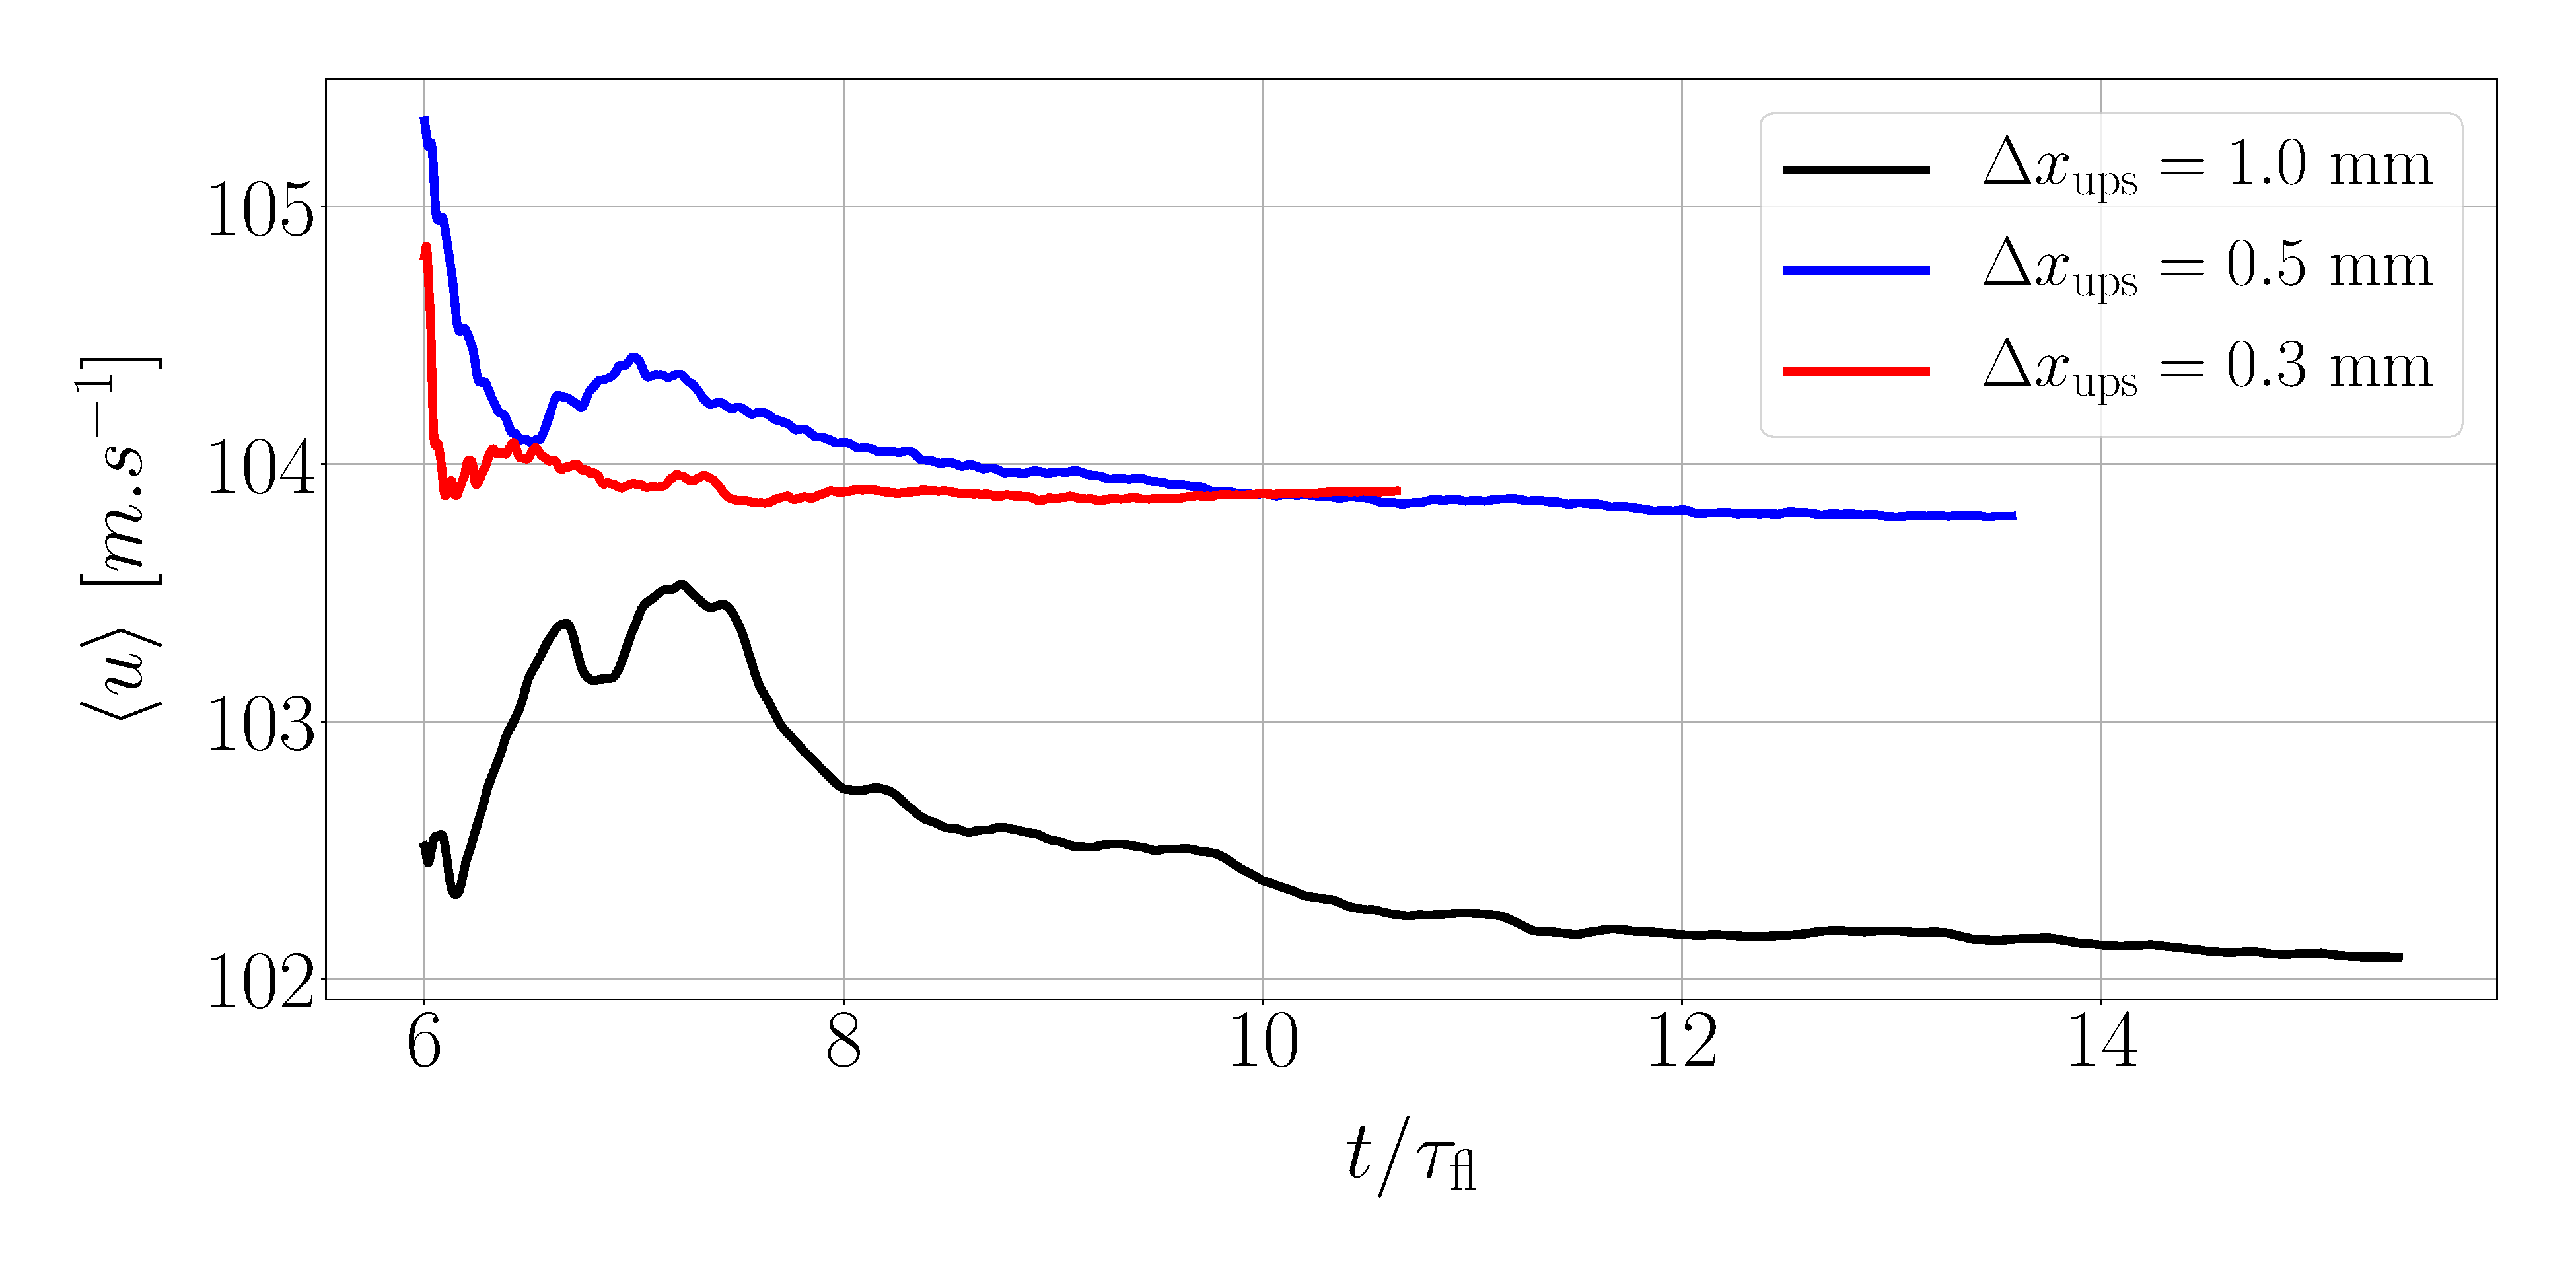
\includegraphics[scale=0.125]{./part2_developments/figures_ch5_resolved_JICF/results_ics_mesh_convergence_line_averages/U_MEAN.pdf}
   \caption{Mean axial velocity}
   %\label{} 
\end{subfigure}
\hfill
\begin{subfigure}[b]{0.45\textwidth}
	\centering
   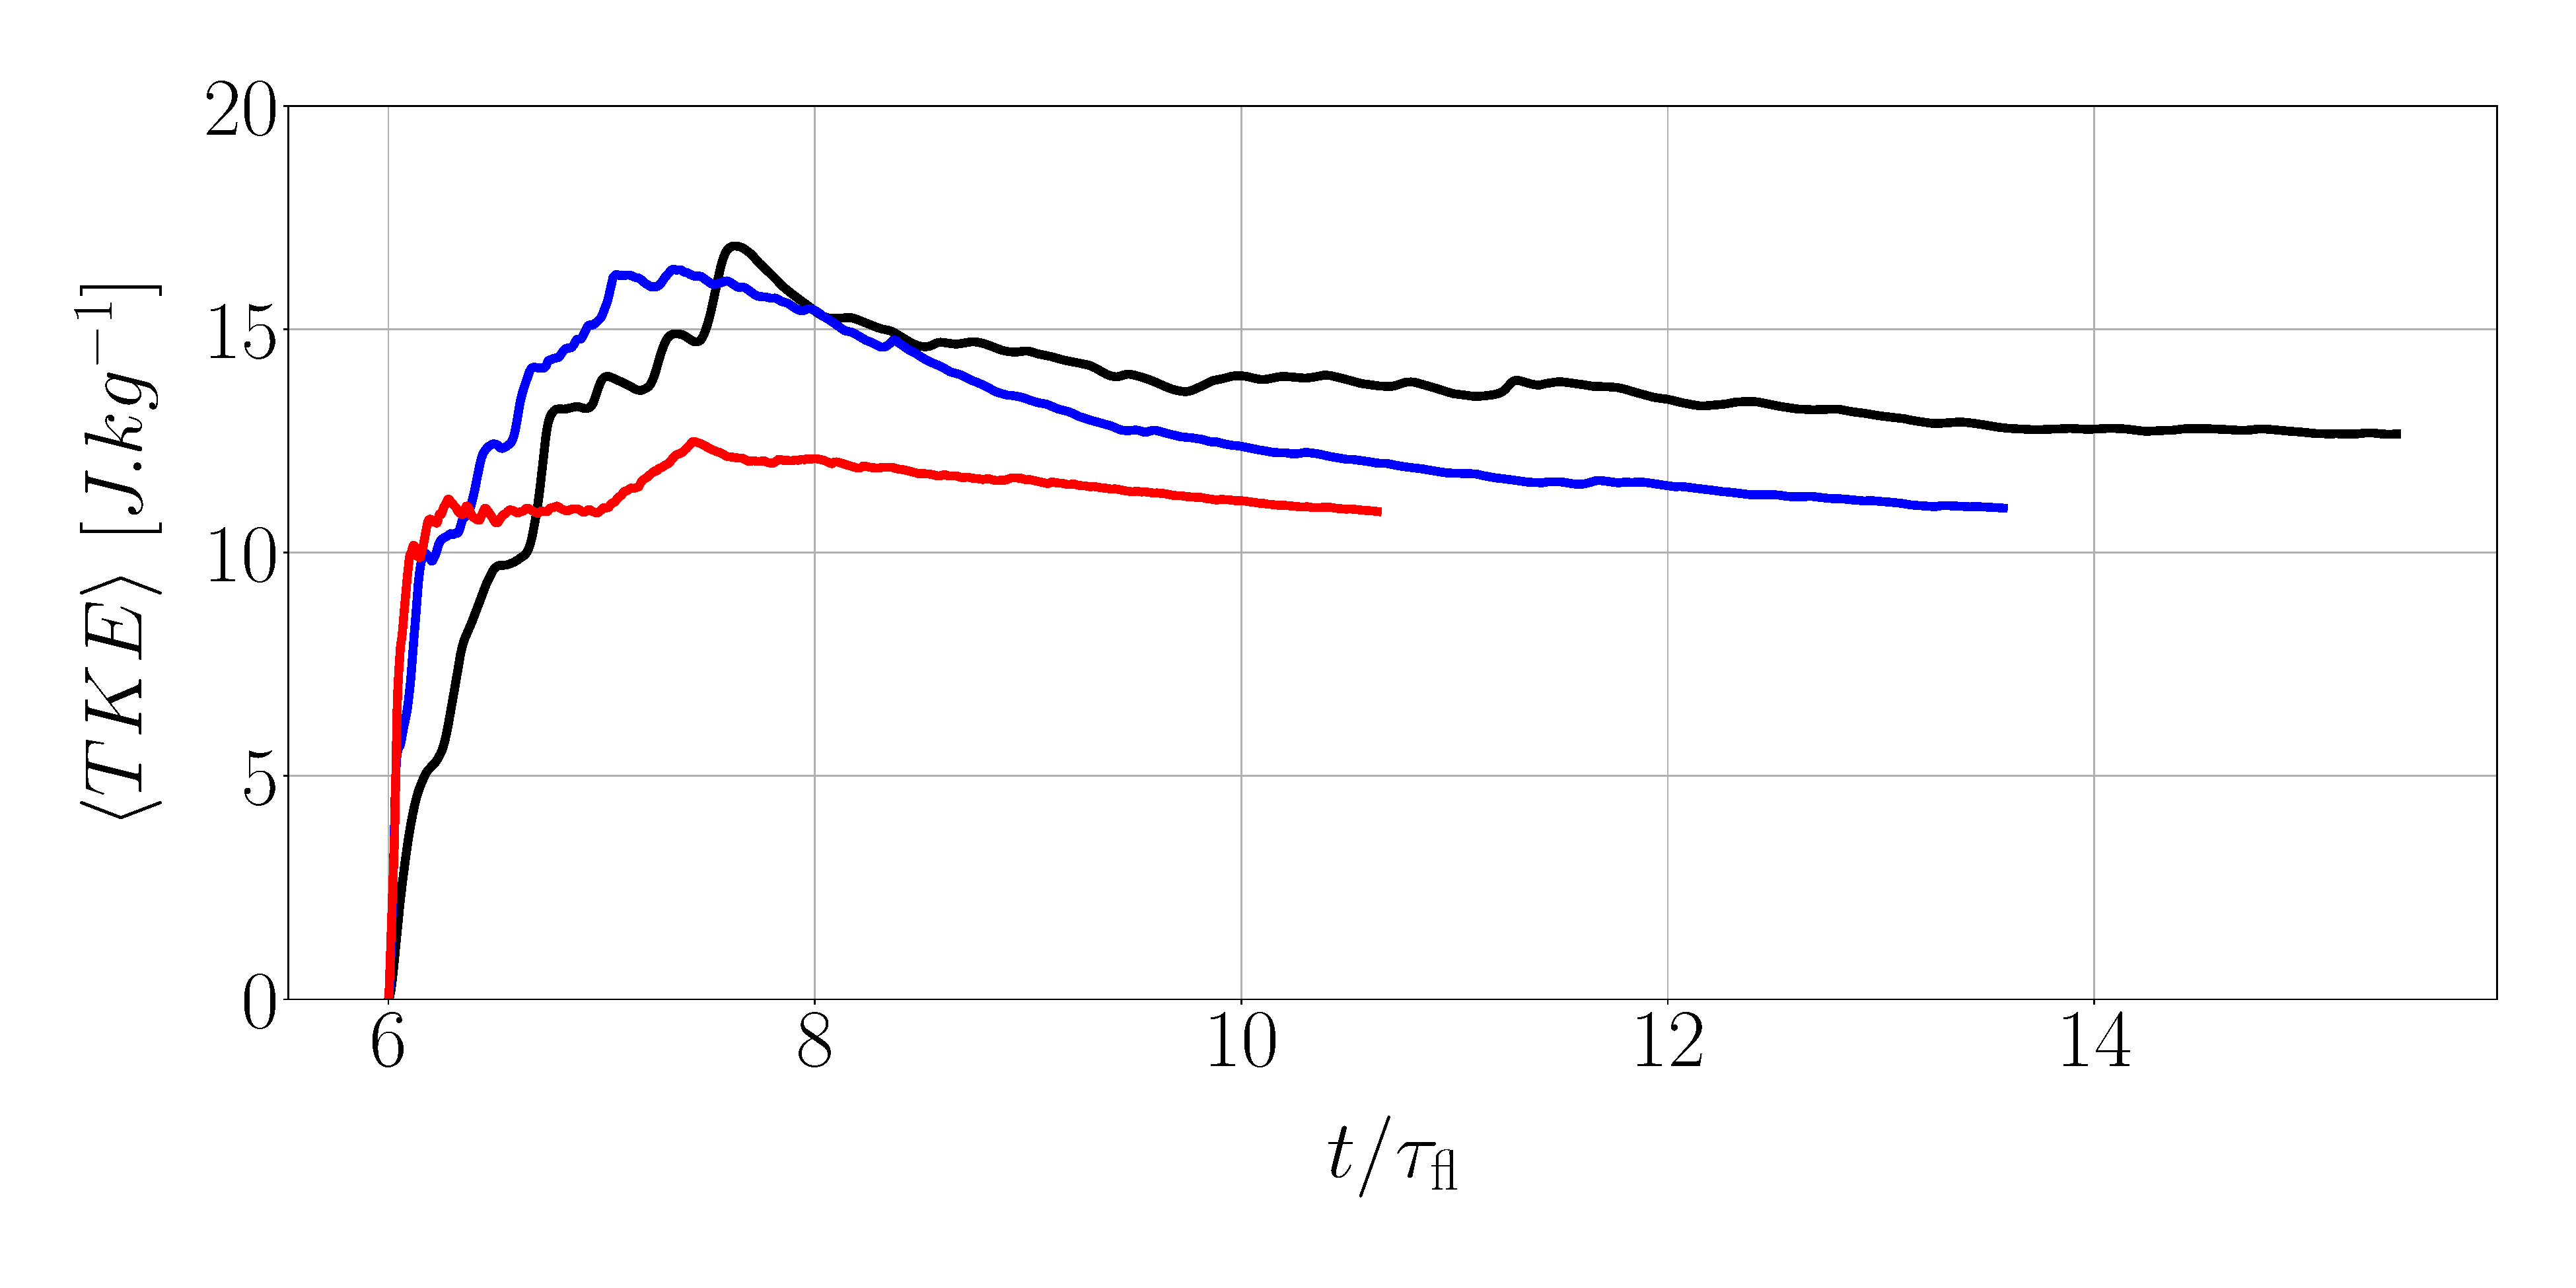
\includegraphics[scale=0.125]{./part2_developments/figures_ch5_resolved_JICF/results_ics_mesh_convergence_line_averages/TKE.pdf}
   \caption{Turbulent Kinetic Energy}
   %\label{}
\end{subfigure}
\caption{Convergence of line-integrated mean axial velocity and TKE with mesh resolution}
\label{fig:mesh_convergence_line_averages}
\end{figure}



Instantaneous snapshots of the fluctuating axial component $u'$ in the middle plane are shown in Figure \ref{fig:ics_mesh_independency_study_up_fields}. The black contours denote the lines with $u' = 0$. As shown, adding turbulence at the inlet introduces fluctuations that are transported downstream the domain. When no turbulence is added, fluctuations are not present (the black contours at the inlet are due to small numerical fluctuations of $u'$) except close to the walls, since they are created inside the boundary layer where flow is turbulent. It is also observed that the characteristic length of the eddies changes when refining the mesh: for the coarsest mesh ($\Delta x_\mathrm{ups} = 1$ mm), these structures are generally large, while refining the mesh to $\Delta x_\mathrm{ups} = 0.5$ and $0.3$ mm reduced their size. 

To assess the quality of the meshes, it is useful to introduce a criterion for measuring the turbulent resolution. For such purpose, the Pope's criterion $M$ is employed \textbf{ref-pope-criterion}, which is calculated from the ratio between the resolved and sub-grid Turbulent Kinetic Energies,  $\mathrm{TKE}$ and $k_\mathrm{sgs}$ respectively:

\begin{equation}
M \left( \textbf{x}, t \right) = \frac{k_\mathrm{sgs} \left( \textbf{x}, t \right)}{k_\mathrm{sgs}  \left( \textbf{x}, t \right) + TKE \left( \textbf{x}, t \right)}
\end{equation}

$M$ represents therefore the ratio between the sub-grid (unresolved) and total TKEs in the domain, and depends on time and space. From its definition it follows that $M = 0$ corresponds to full resolution (i.e. DNS) and $M = 1$ to full modelling (i.e. RANS) of the turbulent flow field. The sub-grid TKE can be obtained from the following expression:


\begin{equation}
k_\mathrm{sgs} = \left( \frac{\nu_t}{0.18 \Delta x} \right)^2
\end{equation}

where $\nu_t$ is the turbulent kinematic viscosity as given by the dynamic Smagorinsky model \citepColor[germano_dynamic_1991]. 

Figure \ref{fig:ics_mesh_independency_study_POPE_M_fields} shows instantenous fields of Pope's criterion for the four simulations performed. As observed, by reducing the element size more regions with values of $M$ closer to $0$ are present. For $\Delta x = 1$ mm there several zones where $M$ has high values. These ones are overall reduced when reducing the cell size to $0.5$ mm and further to $0.3$ mm. Between these last two cell sizes there are also differences in the $M$ field specially far from the walls. For all cases, the $M$ values close to the walls are higher than in the far-field, indicating that a finer resolution would be needed in the walls to properly capture the turbulent features of the boundary layer. Nevertheless, these ones remain around $M \approx 0.5$ for the meshes with $\Delta x = 0.5$ and $0.3$ mm, indicating enough resolution for LES simulations. Regarding the case without turbulence injection for $\Delta x = 0.5$ mm, the $M$ field shows higher values with respect to the case where turbulence is added, specially closer to the inlet and in the regions outside the boundary layer. 

In order to compare quantitatively the difference between meshes, the signals of $u'$ have been monitored with time at the probes shown by the white crosses in the top of Figure \ref{fig:ics_mesh_independency_study_up_fields}. Two probes have been located: one at 1 mm downstream the gaseous inlet (x = 1 mm) and another one 1 mm upstream the liquid injection nozzle (x = 119 mm), both at a height of 8 mm from the bottom walls. The capability of the meshes to transport the resolved turbulent scales, which is of the order of the turbulent fluctuations displayed in Table \ref{tab:jicf_operating_conditions_turbulent_injection_parameters}, is then verified by comparing the fluctuations and spectra obtained with Fast Fourier Transform (FFT) at both probes in Figure \ref{fig:ics_mesh_independency_study_probes}. Time has been normalised with the flow-through time $\tau_\mathrm{fl}$, and the signals are shown for one passage of $\tau_\mathrm{fl}$ for easiness of visualization. For the coarsest mesh $\Delta x_\mathrm{ups} = 1$ mm (Figure \ref{fig:ics_mesh_independency_study_probes_dx1p0}), the $u'$ sampled closer to the nozzle show similar magnitudes but different frequencies to the one from upstream. The spectra confirms this observation: the FFT of probe A displays clearly dominant frequencies at 8, 17 and 25 $\mathrm{kHz}$ with decreasing intensity, while probe A shows also peaks at these locations but also a high predominance of small frequencies. This shows that the mesh with $\Delta x_\mathrm{ups} = 1$ mm is not fully capable of properly transporting the frequencies of the fluctuations. When the mesh is refined to $\Delta x_\mathrm{ups} = 0.5$ mm (Figure \ref{fig:ics_mesh_independency_study_probes_dx0p5}), the small dominant frequencies are no longer relevant and the dominant frequencies are properly captured, as the match in the peaks of the spectra indicate. In this case, the frequencies 8 and 25 $\mathrm{kHz}$ have larger intensity than 17 $\mathrm{kHz}$ . Refining the mesh to $\Delta x_\mathrm{ups} = 0.3$ mm (Figure \ref{fig:ics_mesh_independency_study_probes_dx0p3}) has no longer effect neither in the magnitude of the fluctuations nor in the spectrum. Finally, the fluctuations and FFT of the simulation performed without turbulence injection for the resolution $\Delta x_\mathrm{ups} = 0.5$ mm is shown Figure \ref{fig:ics_mesh_independency_study_probes_dx0p5_no_turb}. As expected, the frequency of the fluctuations  for probe A is minimal (not observed in the $u'$ graph) and predominant frequencies are low. Further downstream some turbulence develops along the channel and created small fluctuations where no clear dominant frequencies are excited. 

\clearpage

\begin{figure}[ht]
\centering
\includeinkscape[inkscapelatex=false,scale=0.75]{./part2_developments/figures_ch5_resolved_JICF/results_ics_mesh_convergence_mesh_and_up/up_field_instantaneous_both}
\caption[Instantaneous $u'$ fields from gaseous simulation for the high Weber case]{Instantaneous $u'$ fields from gaseous simulation for the high Weber case. The right column shows a zoomed-in view of the dashed rectangle from the left column. The black contours indicate the lines with zero instantaneous fluctuation $u' = 0$. From top to bottom $\Delta x_\mathrm{ups} = 1, 0.5, 0.3$ mm.}
\label{fig:ics_mesh_independency_study_up_fields}
\end{figure}

\begin{figure}[ht]
\centering
\includeinkscape[inkscapelatex=false,scale=0.75]{./part2_developments/figures_ch5_resolved_JICF/results_ics_mesh_convergence_POPE/pope_instantaneous_all}
\caption[]{Views of Pope criterion}
\label{fig:ics_mesh_independency_study_POPE_M_fields}
\end{figure}



\begin{figure}[ht]
\centering
\begin{subfigure}[b]{1.0\textwidth}
	\centering   
	\includegraphics[scale=0.28]{./part2_developments/figures_ch5_resolved_JICF/results_ics_mesh_convergence_probes/up_dx1p0.eps}
	\includegraphics[scale=0.28]{./part2_developments/figures_ch5_resolved_JICF/results_ics_mesh_convergence_probes/spectra_linear_scale_dx1p0.eps}
%	\subfloat[\centering]{{\includegraphics[scale=0.20]{./part2_developments/figures_ch5_resolved_JICF/results_ics_mesh_convergence_probes/up_dx1p0.eps} }}%
%    \qquad
%    \subfloat[\centering]{{ \includegraphics[scale=0.20]{./part2_developments/figures_ch5_resolved_JICF/results_ics_mesh_convergence_probes/spectra_linear_scale_dx1p0.eps} }}%
   \caption{Mesh $\Delta x_\mathrm{ups} = 1$ mm}
   \label{fig:ics_mesh_independency_study_probes_dx1p0}
\end{subfigure}


\vskip\baselineskip

\begin{subfigure}[b]{1.0\textwidth}
	\centering
   \includegraphics[scale=0.28]{./part2_developments/figures_ch5_resolved_JICF/results_ics_mesh_convergence_probes/up_dx0p5.eps}
   \includegraphics[scale=0.28]{./part2_developments/figures_ch5_resolved_JICF/results_ics_mesh_convergence_probes/spectra_linear_scale_dx0p5.eps}
   \caption{Mesh $\Delta x_\mathrm{ups} = 0.5$ mm}
   \label{fig:ics_mesh_independency_study_probes_dx0p5}
\end{subfigure}

\vskip\baselineskip

\begin{subfigure}[b]{1.0\textwidth}
	\centering
   \includegraphics[scale=0.28]{./part2_developments/figures_ch5_resolved_JICF/results_ics_mesh_convergence_probes/up_dx0p3.eps}
   \includegraphics[scale=0.28]{./part2_developments/figures_ch5_resolved_JICF/results_ics_mesh_convergence_probes/spectra_linear_scale_dx0p3.eps}
   \caption{{Mesh $\Delta x_\mathrm{ups} = 0.3$ mm}}
   \label{fig:ics_mesh_independency_study_probes_dx0p3}
\end{subfigure}


\vskip\baselineskip

\begin{subfigure}[b]{1.0\textwidth}
	\centering
   \includegraphics[scale=0.28]{./part2_developments/figures_ch5_resolved_JICF/results_ics_mesh_convergence_probes/up_dx0p5_no_turb.eps}
   \includegraphics[scale=0.28]{./part2_developments/figures_ch5_resolved_JICF/results_ics_mesh_convergence_probes/spectra_linear_scale_dx0p5_no_turb.eps}
   \caption{Mesh $\Delta x_\mathrm{ups} = 0.5$ mm without turbulence injection}
   \label{fig:ics_mesh_independency_study_probes_dx0p5_no_turb}
\end{subfigure}

\caption[Frequential analysis of the fluctuations at the sampling probes for the simulations at high Weber number.]{Frequential analysis of the fluctuations at the sampling probes for the simulations at high Weber number. \textsl{Left}: $u'$ fluctuations. \textsl{Right}: spectra of the fluctuations obtained through FFT.}
\label{fig:ics_mesh_independency_study_probes}
\end{figure}




Finally, the profiles of mean axial velocity $\overline{u}$ and TKE are plotting along the vertical line shown in Figure \ref{fig:ics_mesh_independency_study_up_fields} right for the half-width of the channel. The results are shown in Figure \ref{fig:ics_mesh_independency_study_mean_profiles}. 












\clearpage


%\begin{figure}[ht]
%\centering
%\begin{subfigure}[b]{0.3\textwidth}
%	\centering
%   \includegraphics[scale=0.20]{./part2_developments/figures_ch5_resolved_JICF/results_ics_mesh_convergence_probes/up_dx1p0.eps}
%   %\caption{}
%   %\label{} 
%\end{subfigure}
%\hfill
%\begin{subfigure}[b]{0.3\textwidth}
%	\centering
%   \includegraphics[scale=0.20]{./part2_developments/figures_ch5_resolved_JICF/results_ics_mesh_convergence_probes/up_dx0p5.eps}
%   %\caption{}
%   %\label{} 
%\end{subfigure}
%\hfill
%\begin{subfigure}[b]{0.3\textwidth}
%	\centering
%   \includegraphics[scale=0.20]{./part2_developments/figures_ch5_resolved_JICF/results_ics_mesh_convergence_probes/up_dx0p3.eps}
%   %\caption{}
%   %\label{} 
%\end{subfigure}
%
%\vskip\baselineskip
%
%\begin{subfigure}[b]{0.3\textwidth}
%	\centering
%   \includegraphics[scale=0.20]{./part2_developments/figures_ch5_resolved_JICF/results_ics_mesh_convergence_probes/spectra_linear_scale_dx1p0.eps}
%   \caption{}
%   %\label{}
%\end{subfigure}
%\hfill
%\begin{subfigure}[b]{0.3\textwidth}
%	\centering
%   \includegraphics[scale=0.20]{./part2_developments/figures_ch5_resolved_JICF/results_ics_mesh_convergence_probes/spectra_linear_scale_dx0p5.eps}
%   \caption{}
%   %\label{}
%\end{subfigure}
%\hfill
%\begin{subfigure}[b]{0.3\textwidth}
%	\centering
%   \includegraphics[scale=0.20]{./part2_developments/figures_ch5_resolved_JICF/results_ics_mesh_convergence_probes/spectra_linear_scale_dx0p3.eps}
%   \caption{}
%   %\label{}
%\end{subfigure}
%
%\caption[YAP]{Probes}
%\label{fig:ics_mesh_independency_study_probes}
%\end{figure}

\clearpage




%\subsection{Effect of injecting turbulence}

%Once the fine mesh has been chosen as the baseline mesh for the , the effect of injecting turbulence is stated. For this, one simulation without turbulence injection is performed for the high Weber case and compared to the simulation with turbulence injection.


\begin{figure}[ht]
\centering
\begin{subfigure}[b]{0.45\textwidth}
	\centering
   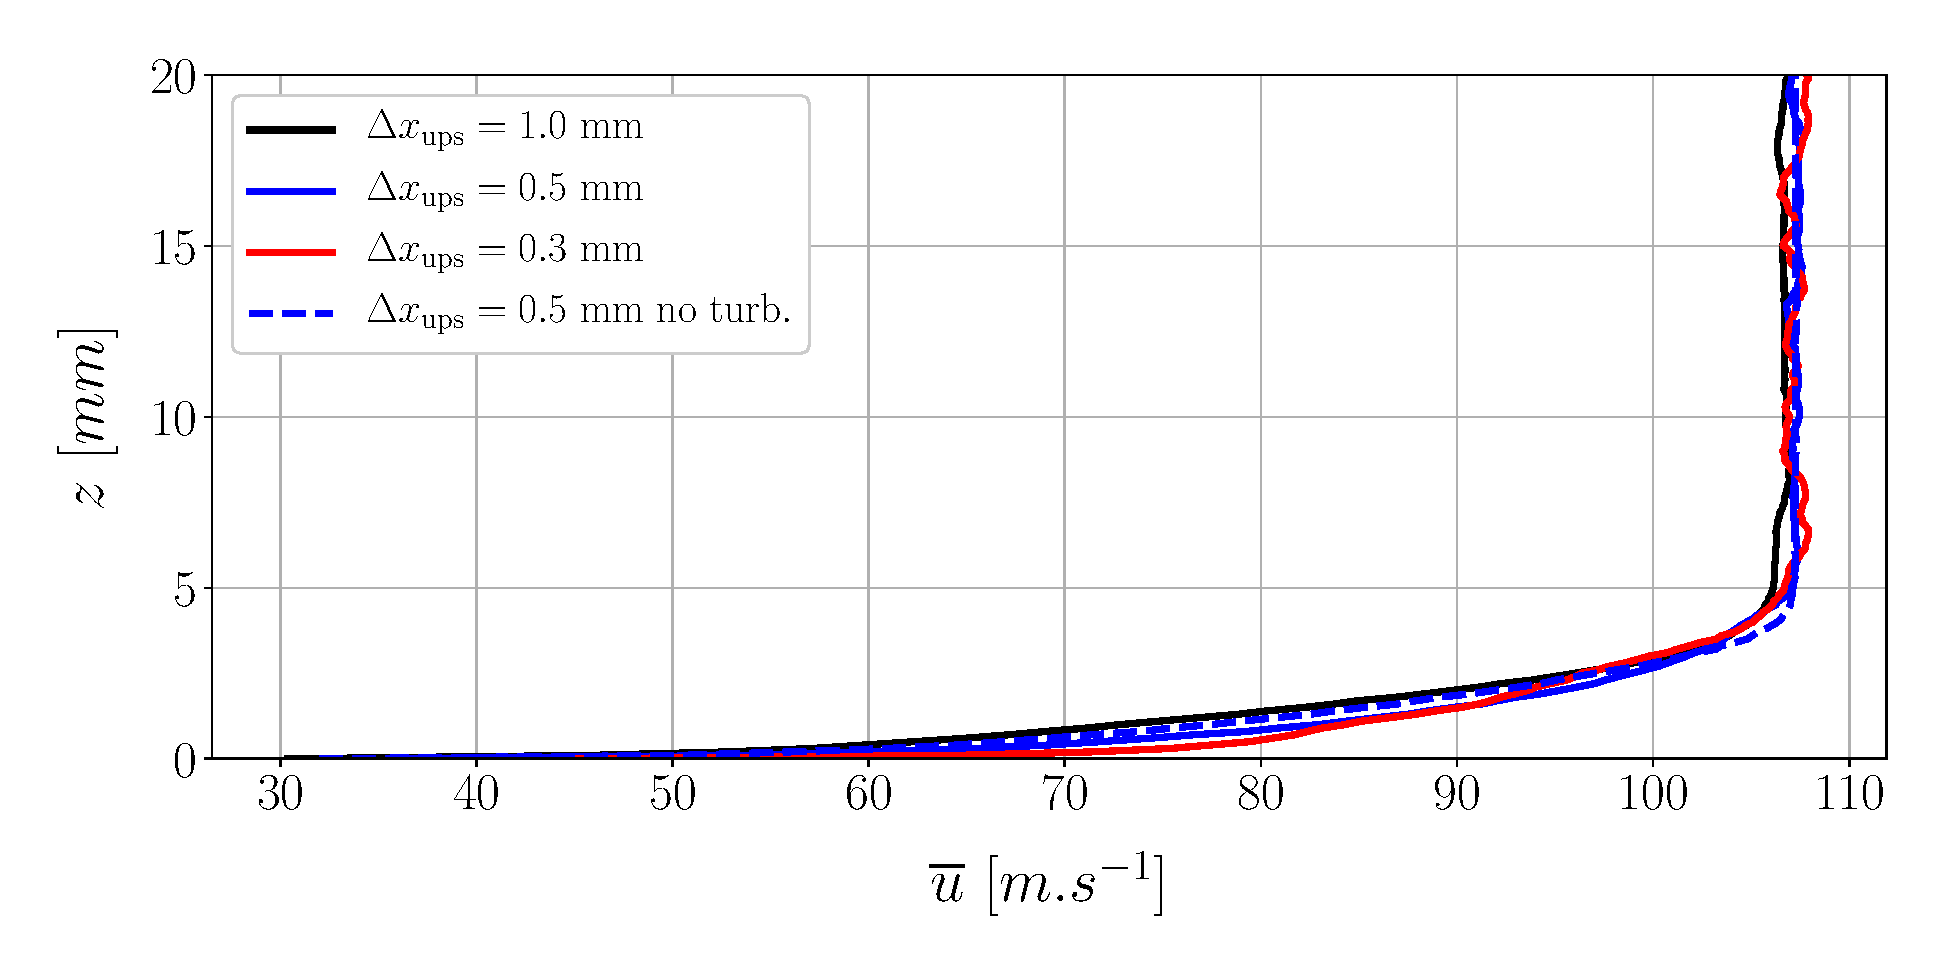
\includegraphics[scale=0.25]{./part2_developments/figures_ch5_resolved_JICF/results_ics_mesh_convergence_mean_profiles/U_MEAN_profiles.pdf}
   \caption{Mean axial velocity}
   %\label{} 
\end{subfigure}
\hfill
\begin{subfigure}[b]{0.45\textwidth}
	\centering
   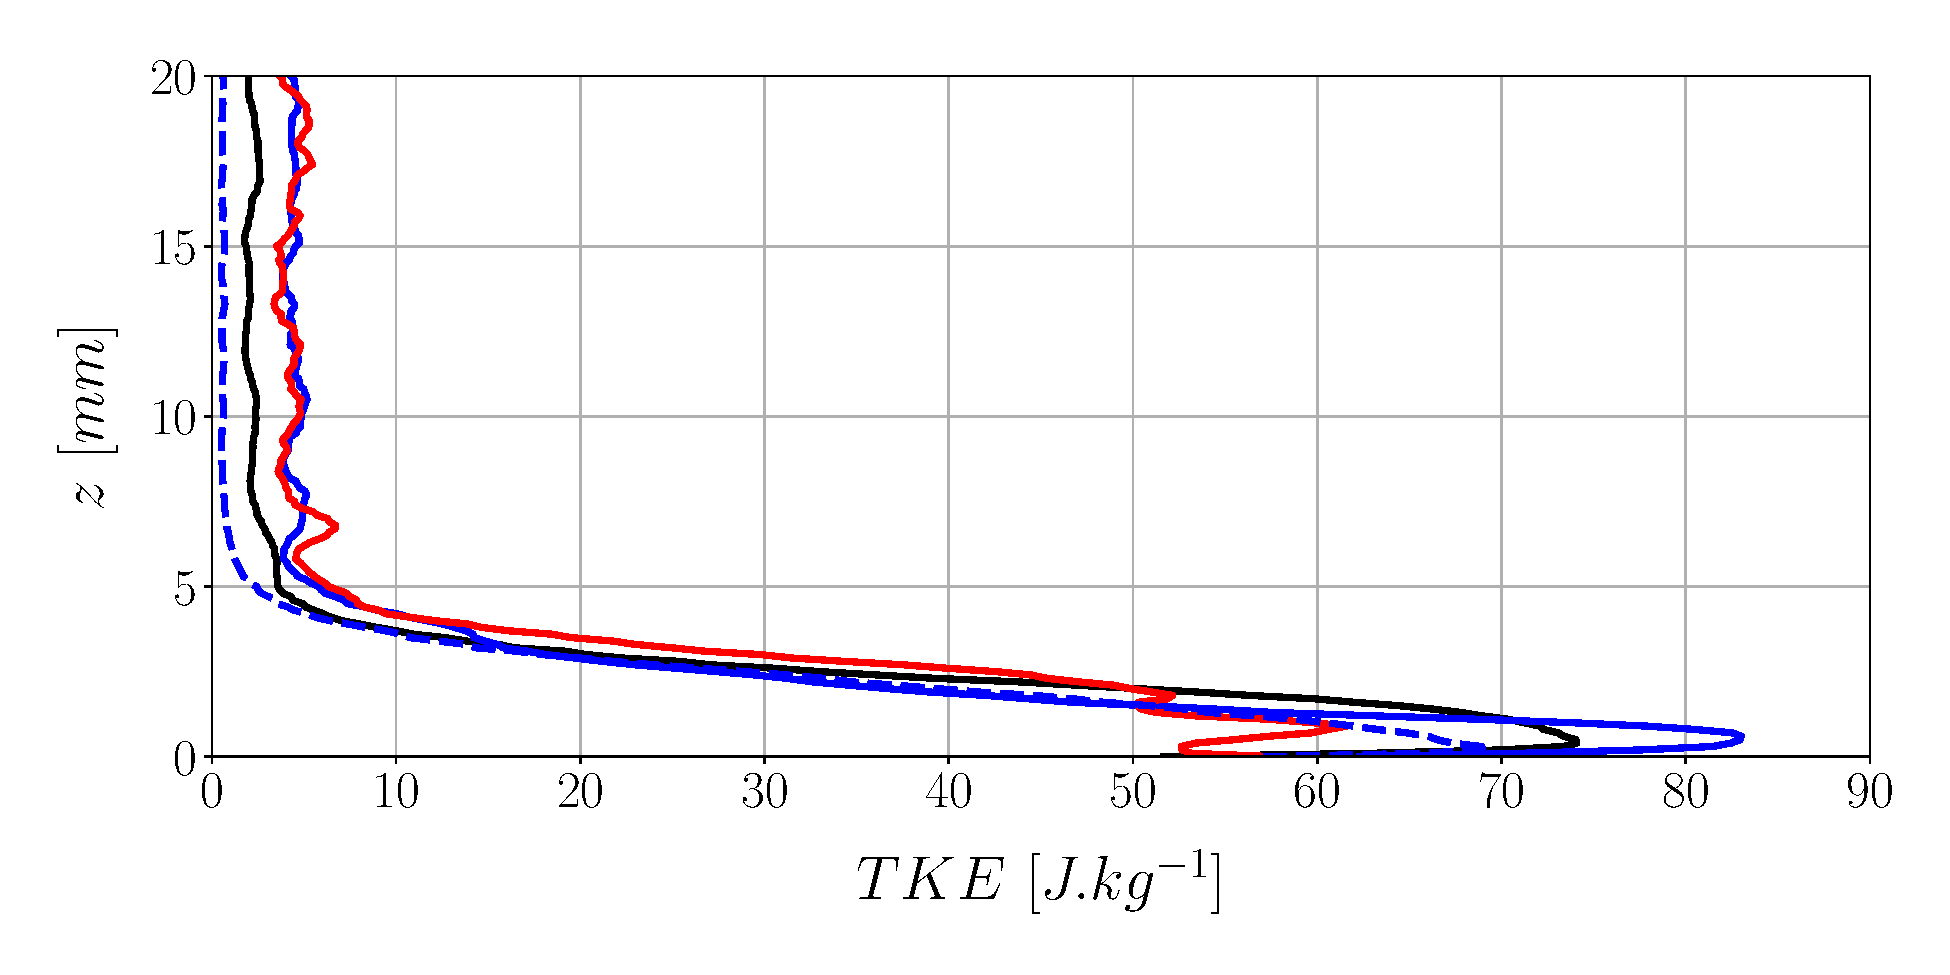
\includegraphics[scale=0.25]{./part2_developments/figures_ch5_resolved_JICF/results_ics_mesh_convergence_mean_profiles/TKE_profiles.pdf}
   \caption{Turbulent Kinetic Energy}
   %\label{}
\end{subfigure}
\caption{Profiles of $\overline{u}$ and $TKE$ along the line right upstream the injector.}
\label{fig:ics_mesh_independency_study_mean_profiles} 
\end{figure}


\subsection{Initial conditions for low Weber operating point}

From the previous analysis, the ...



\begin{figure}[ht]
	\centering
   \includegraphics[scale=0.28]{./part2_developments/figures_ch5_resolved_JICF/results_ics_mesh_convergence_probes/up_OP2.eps}
   \includegraphics[scale=0.28]{./part2_developments/figures_ch5_resolved_JICF/results_ics_mesh_convergence_probes/spectra_linear_scale_OP2.eps}
   \caption{Mesh $\Delta x_\mathrm{ups} = 0.5$ mm, low-We operating point}
   \label{fig:ics_probes_OP2}
\end{figure}




\section{Definition of characteristic times}

In order to analyse the convergence and results of the four simulations performed, it is useful to relate the simulation times to characteristic times relating the liquid. Three characteristic times are considered in this work:

\begin{itemize}
	
	\item $\tau_\mathrm{liq}$: the characteristic liquid phase time from \citeColor[ranger_aerodynamics_1968], defined as:
	
	\begin{equation}
	\tau_\mathrm{liq} = \sqrt{\frac{\rho_l}{\rho_g}} \frac{d_\mathrm{inj}}{u_g}
	\end{equation}
	
	\item $\tau_\mathrm{ph}$: a characteristic physical time of the JICF, defined as )\textbf{ref:herrmann-2011}):
	
	\begin{equation}
	\label{eq:jicf_tau_injector}
	\tau_\mathrm{ph} = \frac{d_\mathrm{inj}}{u_l}
	\end{equation}

	\item $\tau_\mathrm{str}$: the characteristic time from ligaments stripping from the dense core. This value is obtained by counting the number of liquid structures that emanate from the liquid column in a given time period.

\end{itemize}



For each simulation, the different characteristic times are defined in Table \ref{tab:jicf_characteristic times}. The values $\tau_\mathrm{liq}$ and $\tau_\mathrm{ph}$, depend obviously on the operating condition and not on the mesh resolution, since they are have been obtained from mathematical formulas. On the other hand, the characteristic time $\tau_\mathrm{str}$ has been obtained from each simulation and a dependency on the mesh resolution employed can be expected. 

\begin{table}[!h]
\centering
\caption{Characteristic times in JICF simulations}
\begin{tabular}{lccc}
\thickhline
\textbf{Case} & $\tau_\mathrm{liq}$ [ms] & $\tau_\mathrm{ph}$ [ms] & $\tau_\mathrm{str}$ [ms] \\
\thickhline 
UG75\_DX10  & 0.047 & 0.019 & \\
UG75\_DX20  & 0.047 & 0.019 & \\
UG100\_DX10 & 0.063 & 0.026 & \\
UG100\_DX20 & 0.063 & 0.026 & \\
\thickhline
\end{tabular}
\label{tab:jicf_characteristic times}
\end{table}

We can also define characteristic times as droplets reach the sampling planes. For it, we can make a specific table for each case and each plane:

\begin{table}[!h]
\centering
\caption{Characteristic droplet times in JICF simulations}
\begin{tabular}{lcccc}
\thickhline
\textbf{Case} & $x = 5 mm$ & $x = 10 mm$ & $x = 15 mm$  \\
\thickhline 
UG75\_DX10  & 0.1927 & 0.2952 & -  \\
UG75\_DX20  & 0.2347 & 0.3558 & 0.4567 \\
UG100\_DX10 & 0.1437 & 0.2187 & - \\
UG100\_DX20 & 0.1768 & 0.2584 & 0.3628 \\
\thickhline
\end{tabular}
\label{tab:jicf_characteristic_droplet_sampling_times}
\end{table}


%\section{Results}
%\label{sec:results_JICF_resolved}

\section{Jet topology}


\subsection{Flow establishment}

A non-dimensional time can be defined as

\begin{equation}
t^* = \frac{t}{\tau_\mathrm{ph}}
\end{equation}

Or:

\begin{equation}
t^* = \frac{t}{\tau_\mathrm{dr}}
\end{equation}


The increase in mesh elements is seen in Figure \ref{fig:JICF_nelem_increase}.

\begin{figure}[ht]
\centering
	\centering
   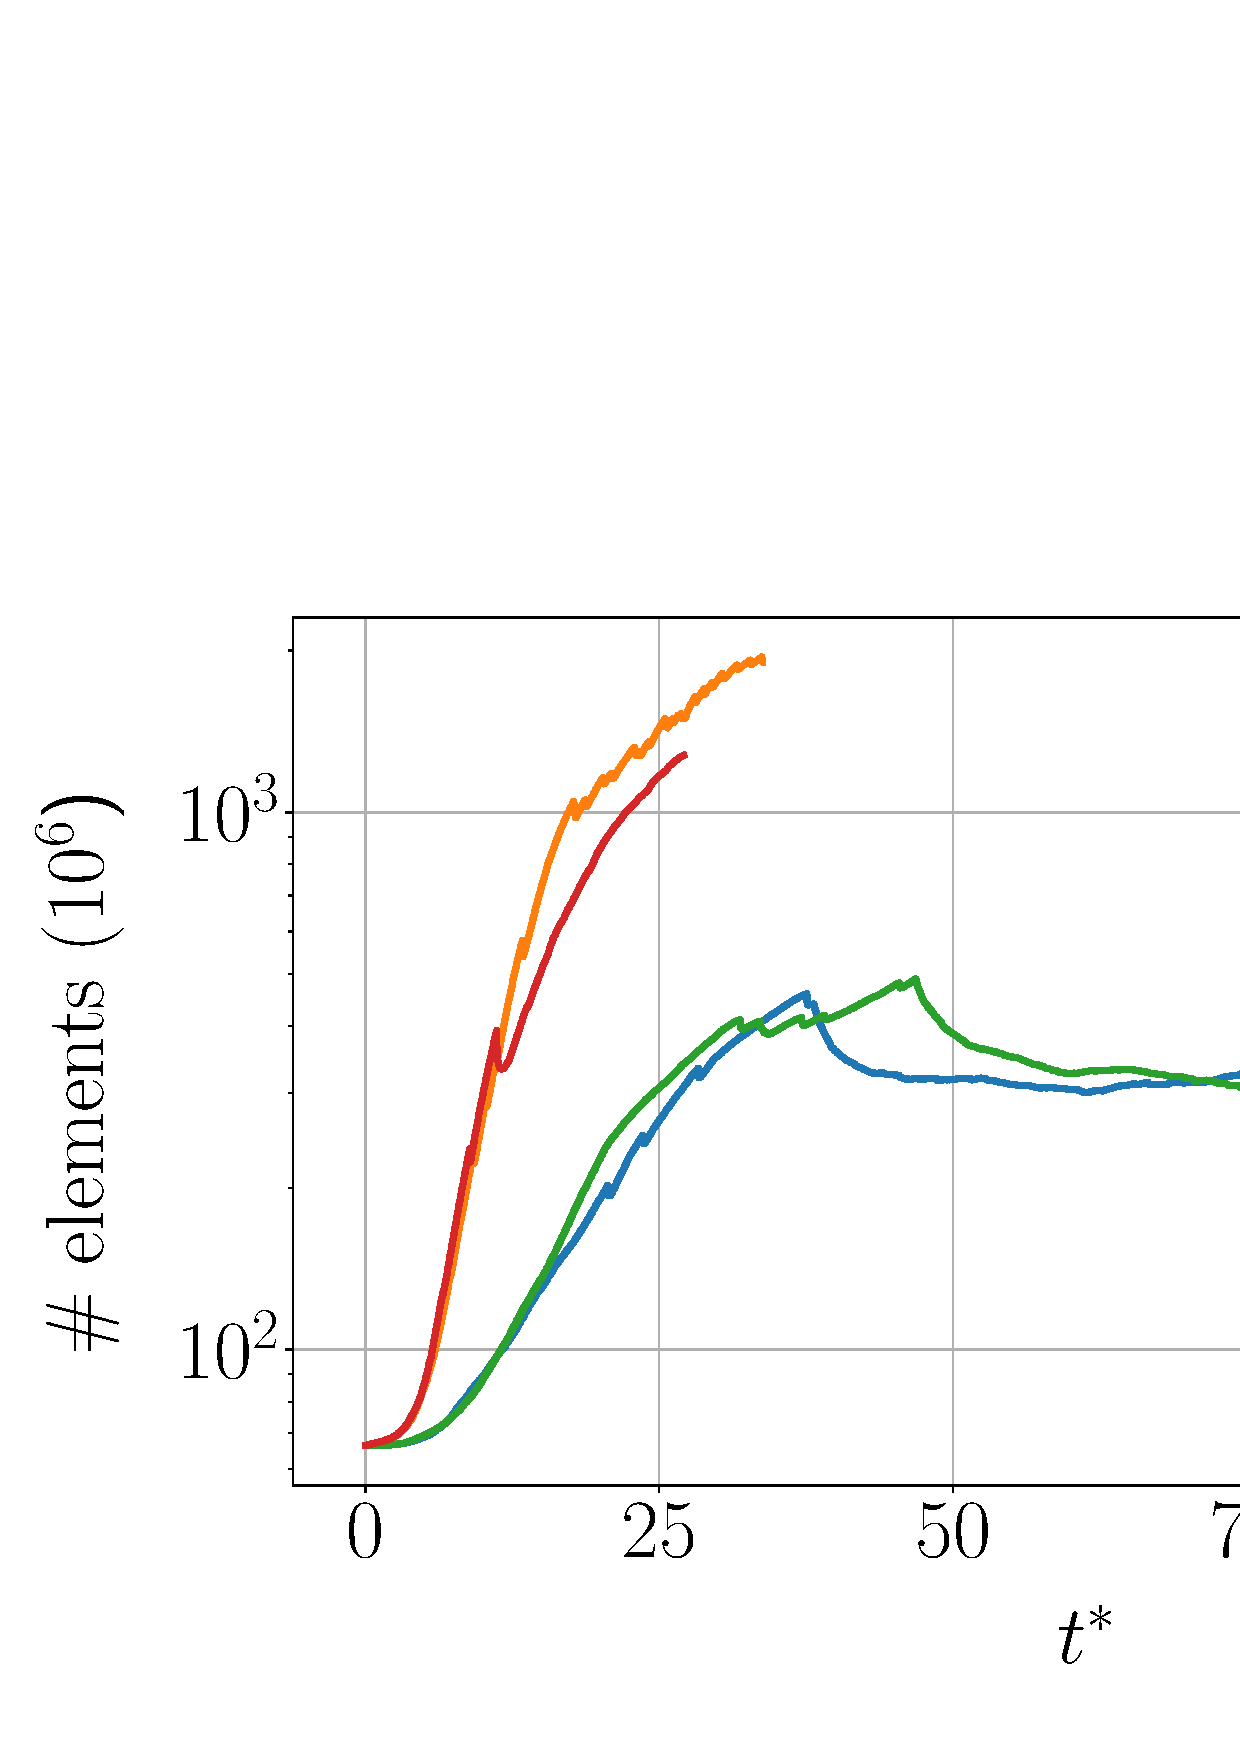
\includegraphics[scale=0.25]{./part2_developments/figures_ch5_resolved_JICF/JICF_nelem_increase}
   %\label{} 
\caption{Evolution of number of mesh elements with time in JICF simulations}
\label{fig:JICF_nelem_increase}
\end{figure}

\clearpage

\begin{figure}[ht]
\centering
\includeinkscape[inkscapelatex=false,scale=0.8]{./part2_developments/figures_ch5_resolved_JICF/JICF_establishment_UG100_lateral}
\caption[Lateral view of high We jet at several time instants. ]{Lateral view of high We jet at several time instants. \textsl{Left}: UG100\_DX20. \textsl{Right}: UG100\_DX10.}
\label{fig:JICF_establishment_UG100_lateral}
\end{figure}

\clearpage

\begin{figure}[ht]
\centering
\includeinkscape[inkscapelatex=false,scale=0.8]{./part2_developments/figures_ch5_resolved_JICF/JICF_establishment_UG100_front}
\caption[Front view of high We jet at several time instants. ]{Front view of high We jet at several time instants. \textsl{Left}: UG100\_DX20. \textsl{Right}: UG100\_DX10.}
\label{fig:JICF_establishment_UG100_front}
\end{figure}
\clearpage

\clearpage

\begin{figure}[ht]
\centering
\includeinkscape[inkscapelatex=false,scale=0.8]{./part2_developments/figures_ch5_resolved_JICF/JICF_establishment_UG100_top}
\caption[Top view of high We jet at several time instants. ]{Top view of high We jet at several time instants. \textsl{Left}: UG100\_DX20. \textsl{Right}: UG100\_DX10.}
\label{fig:JICF_establishment_UG100_top}
\end{figure}




\clearpage

\begin{figure}[ht]
\centering
\includeinkscape[inkscapelatex=false,scale=0.8]{./part2_developments/figures_ch5_resolved_JICF/JICF_establishment_UG75_lateral}
\caption[Lateral view of low We jet at several time instants. ]{Lateral view of low We jet at several time instants. \textsl{Left}: UG75\_DX20. \textsl{Right}: UG75\_DX10.}
\label{fig:JICF_establishment_UG75_lateral}
\end{figure}

\clearpage

\begin{figure}[ht]
\centering
\includeinkscape[inkscapelatex=false,scale=0.8]{./part2_developments/figures_ch5_resolved_JICF/JICF_establishment_UG75_front}
\caption[Front view of low We jet at several time instants. ]{Front view of low We jet at several time instants. \textsl{Left}: UG75\_DX20. \textsl{Right}: UG75\_DX10.}
\label{fig:JICF_establishment_UG75_front}
\end{figure}

\clearpage

\begin{figure}[ht]
\centering
\includeinkscape[inkscapelatex=false,scale=0.8]{./part2_developments/figures_ch5_resolved_JICF/JICF_establishment_UG75_top}
\caption[Top view of low We jet at several time instants. ]{Top view of low We jet at several time instants. \textsl{Left}: UG75\_DX20. \textsl{Right}: UG75\_DX10.}
\label{fig:JICF_establishment_UG75_top}
\end{figure}

\clearpage

\subsection{Jet breakup}


\section{Jet trajectories}
\label{subsec:ch5_jet_trajectories_results}

Different methods to obtain trajectories from resolved simulations were proposed in $\S$\ref{sec:ch5_tools_jicf_trajectories}. These methods are summarized in Table \ref{tab:jicf_tools_trajectories_obtention}. In this section, firstly  the four methods described are applied to the simulation UG100\_DX20, the trajectories obtained are then compared and discussed. Secondly, the method MEAN\_GRAD is chosen to perform experimental validation with all simulations from Table \ref{tab:jicf_resolved_simulations_performed}, since this is the numerical methodology more similar to the way in which the experimental correlations in \citeColor[becker_breakup_2002] are obtained.

The accuracy of the mean numerical trajectories can be quantitatively assessed by defining a $L_2$ error as in Eq.~(\ref{eq:L2_JICF}): 

\begin{equation}
\label{eq:L2_JICF}
    L_2 = \sqrt{\frac{1}{N}   \sum_{i=1}^N \left( \frac{z}{d_\mathrm{inj}} \Bigr|_{\mathrm{num},i} -   \frac{z}{d_\mathrm{inj}} \Bigr|_{\mathrm{exp},i} \right)^2}
\end{equation}



We can also define an error along the trajectory as follows:



\begin{equation}
\varepsilon_i  =  \frac{ \frac{z}{d_\mathrm{inj}} \Bigr|_{\mathrm{num},i} - \frac{z}{d_\mathrm{inj}} \Bigr|_{\mathrm{exp},i} }{ \frac{z}{d_\mathrm{inj}} \Bigr|_{\mathrm{exp},i} }
\end{equation}

\begin{equation}
\varepsilon_i  =  \frac{ z/d_\mathrm{inj} \Bigr|_{\mathrm{num},i} - z/d_\mathrm{inj} \Bigr|_{\mathrm{exp},i} }{ z/d_\mathrm{inj} \Bigr|_{\mathrm{exp},i} }
\end{equation}


\subsection{Comparison of methods}


\begin{figure}[ht]
\centering
\begin{subfigure}[b]{0.45\textwidth}
	\centering
   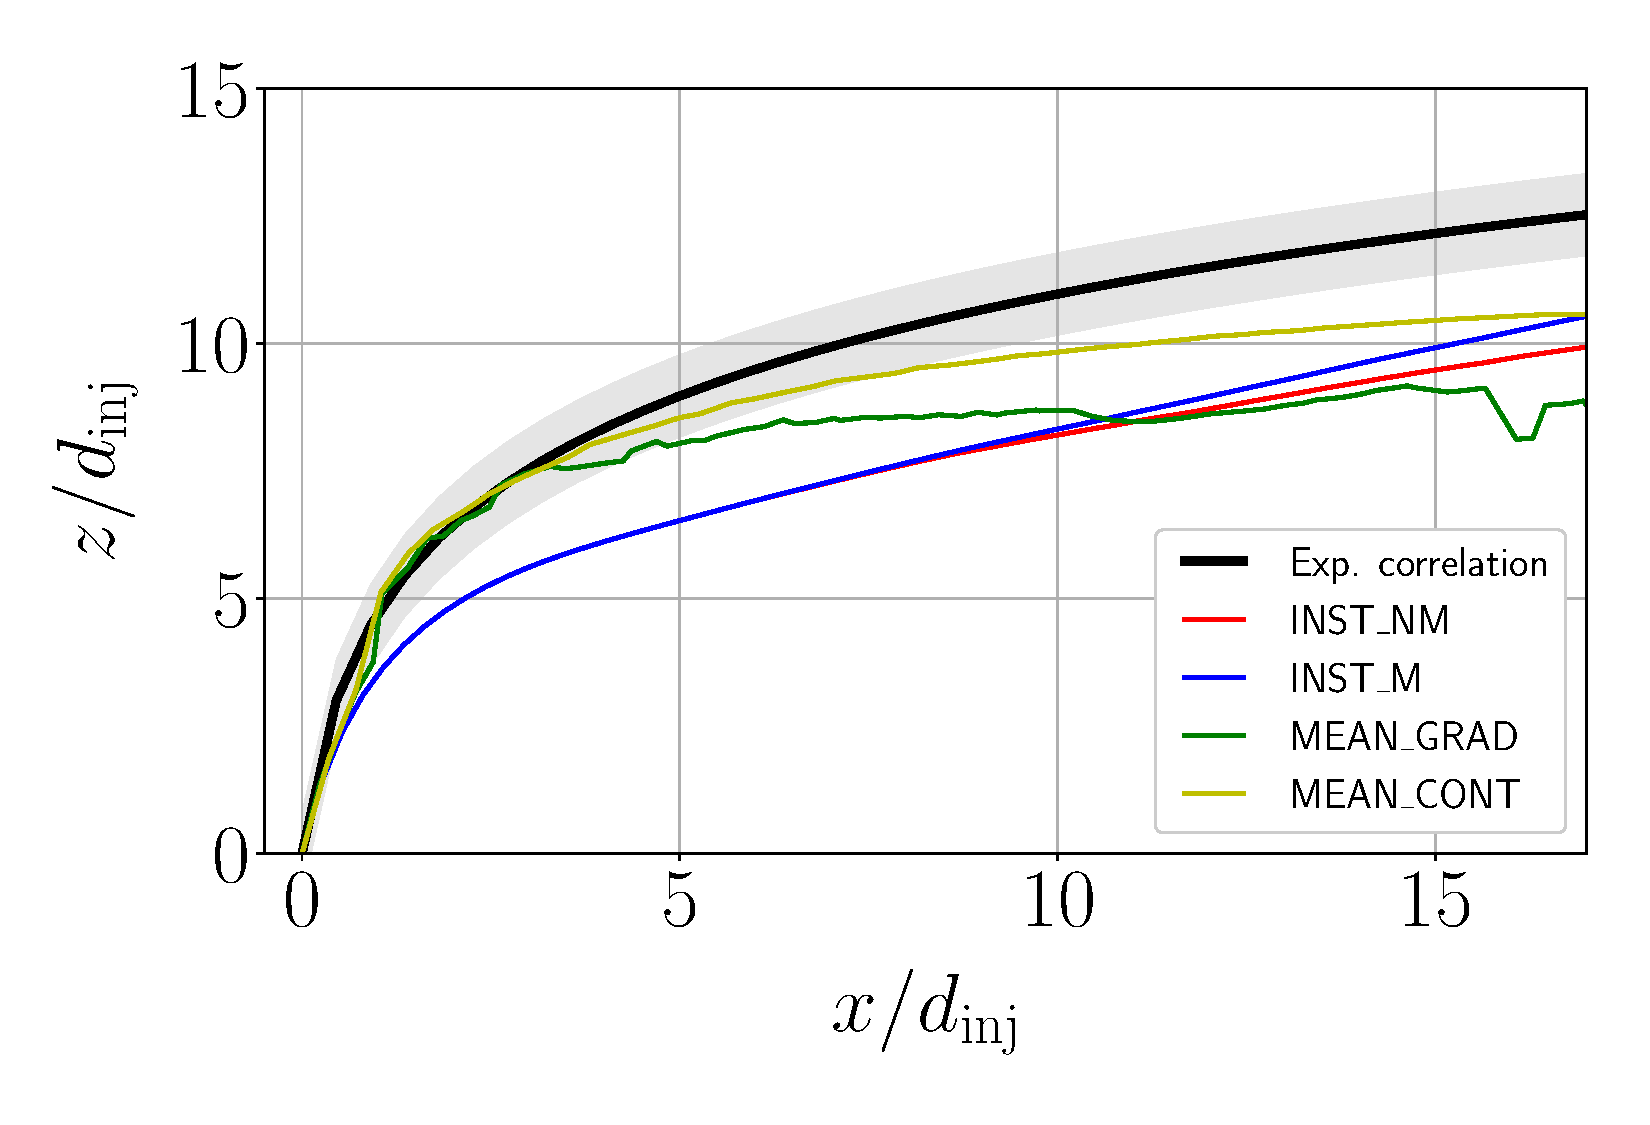
\includegraphics[scale=0.15]{./part2_developments/figures_ch5_resolved_JICF/results_trajectories/methods_comparison_trajectories_q6uG100.pdf}
   \caption{Mean trajectories}
   %\label{} 
\end{subfigure}
\hfill
\begin{subfigure}[b]{0.45\textwidth}
	\centering
   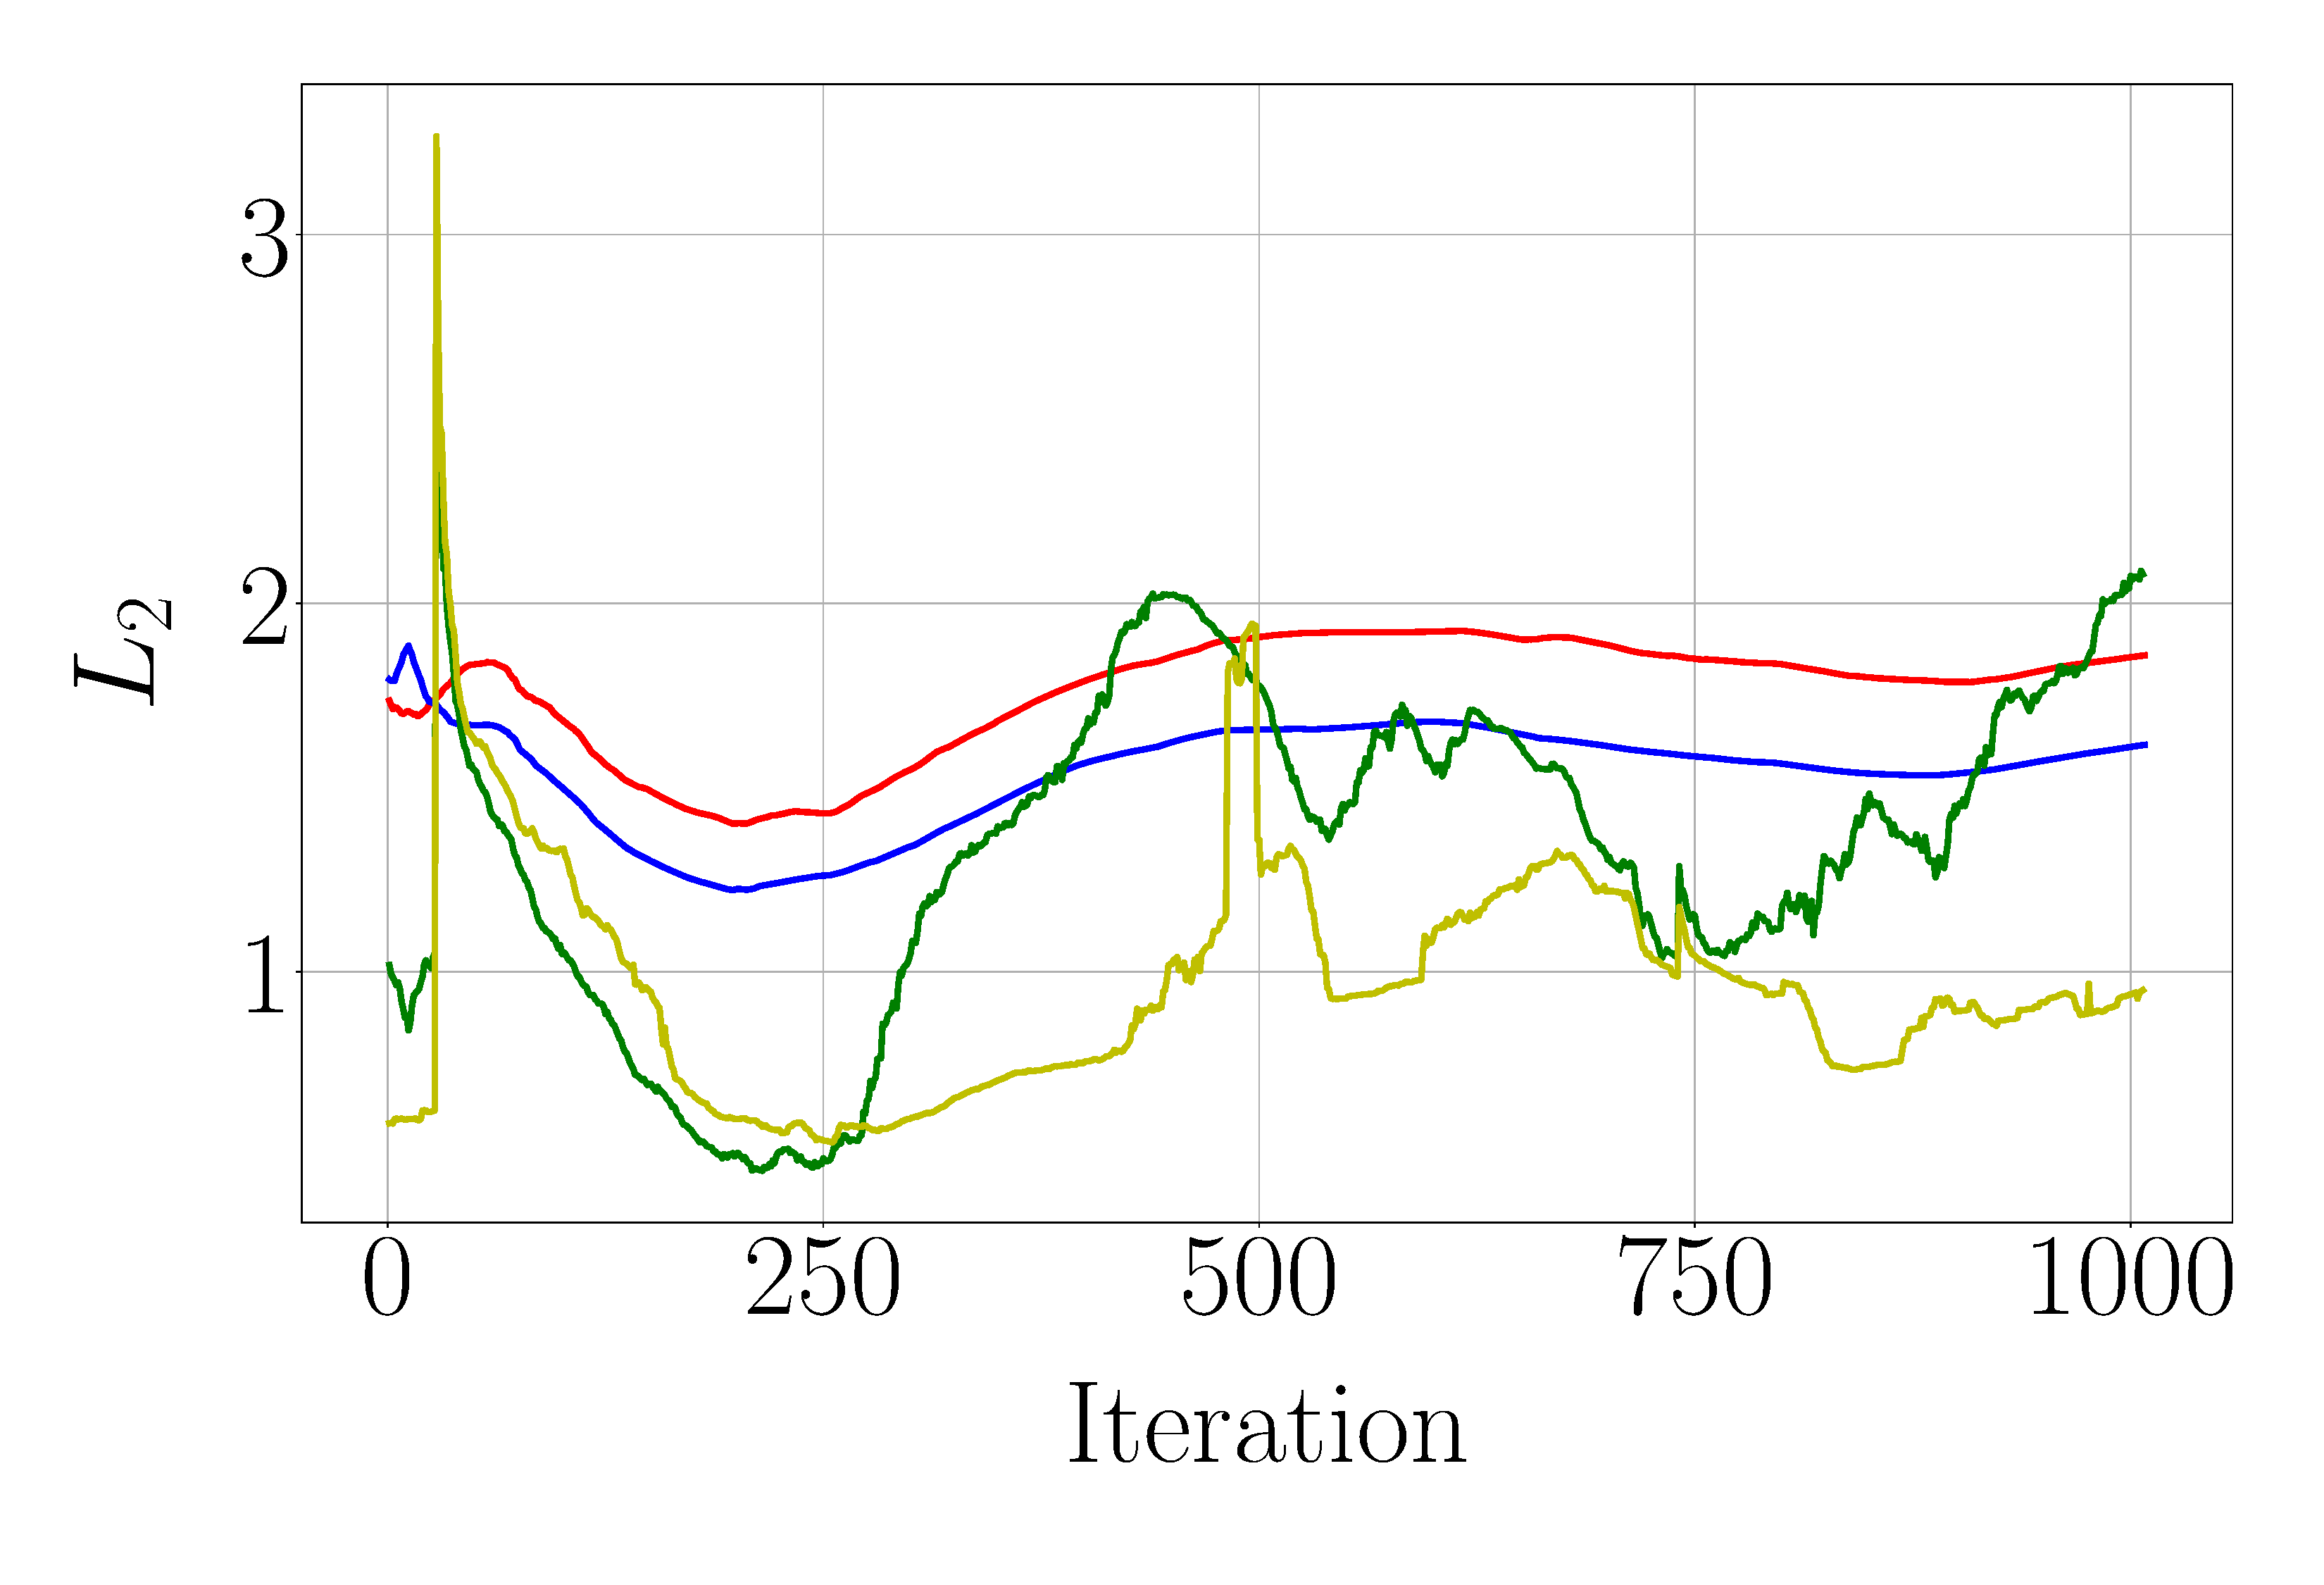
\includegraphics[scale=0.15]{./part2_developments/figures_ch5_resolved_JICF/results_trajectories/methods_comparison_L2_evolution_q6uG100.pdf}
   \caption{$L_2$ error evolution}
   %\label{}
\end{subfigure}
\caption{Trajectories and $L_2$ errors obtained with different methods for case UG100\_DX20}
\label{fig:JICF_trajectories_and_L2_comparison}
\end{figure}

\subsection{Experimental validation}

\begin{figure}[ht]
\centering
\begin{subfigure}[b]{0.45\textwidth}
	\centering
   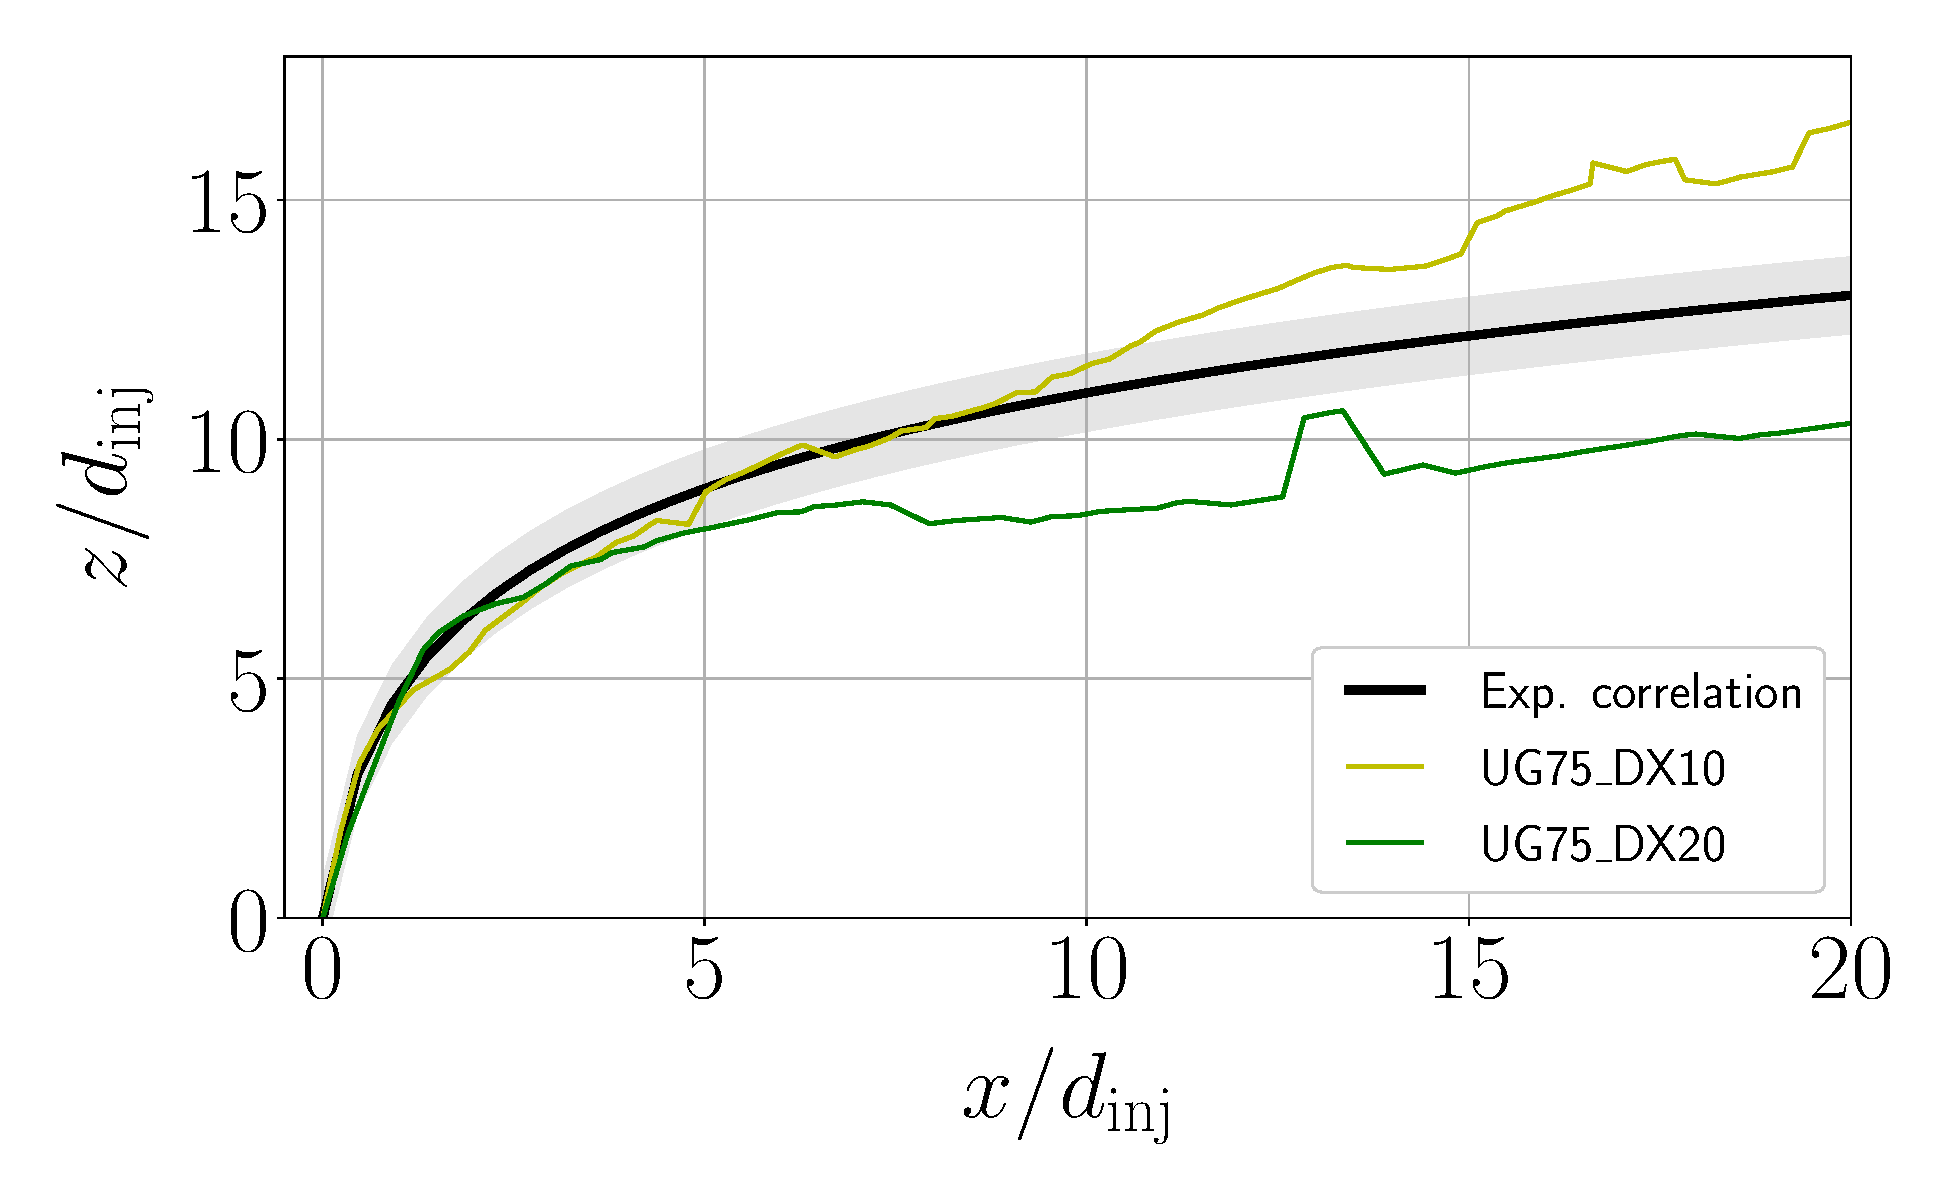
\includegraphics[scale=0.15]{./part2_developments/figures_ch5_resolved_JICF/results_trajectories/methods_expe_validation_trajectories_q6uG75.pdf}
   \caption{Low $We$}
   %\label{} 
\end{subfigure}
\hfill
\begin{subfigure}[b]{0.45\textwidth}
	\centering
   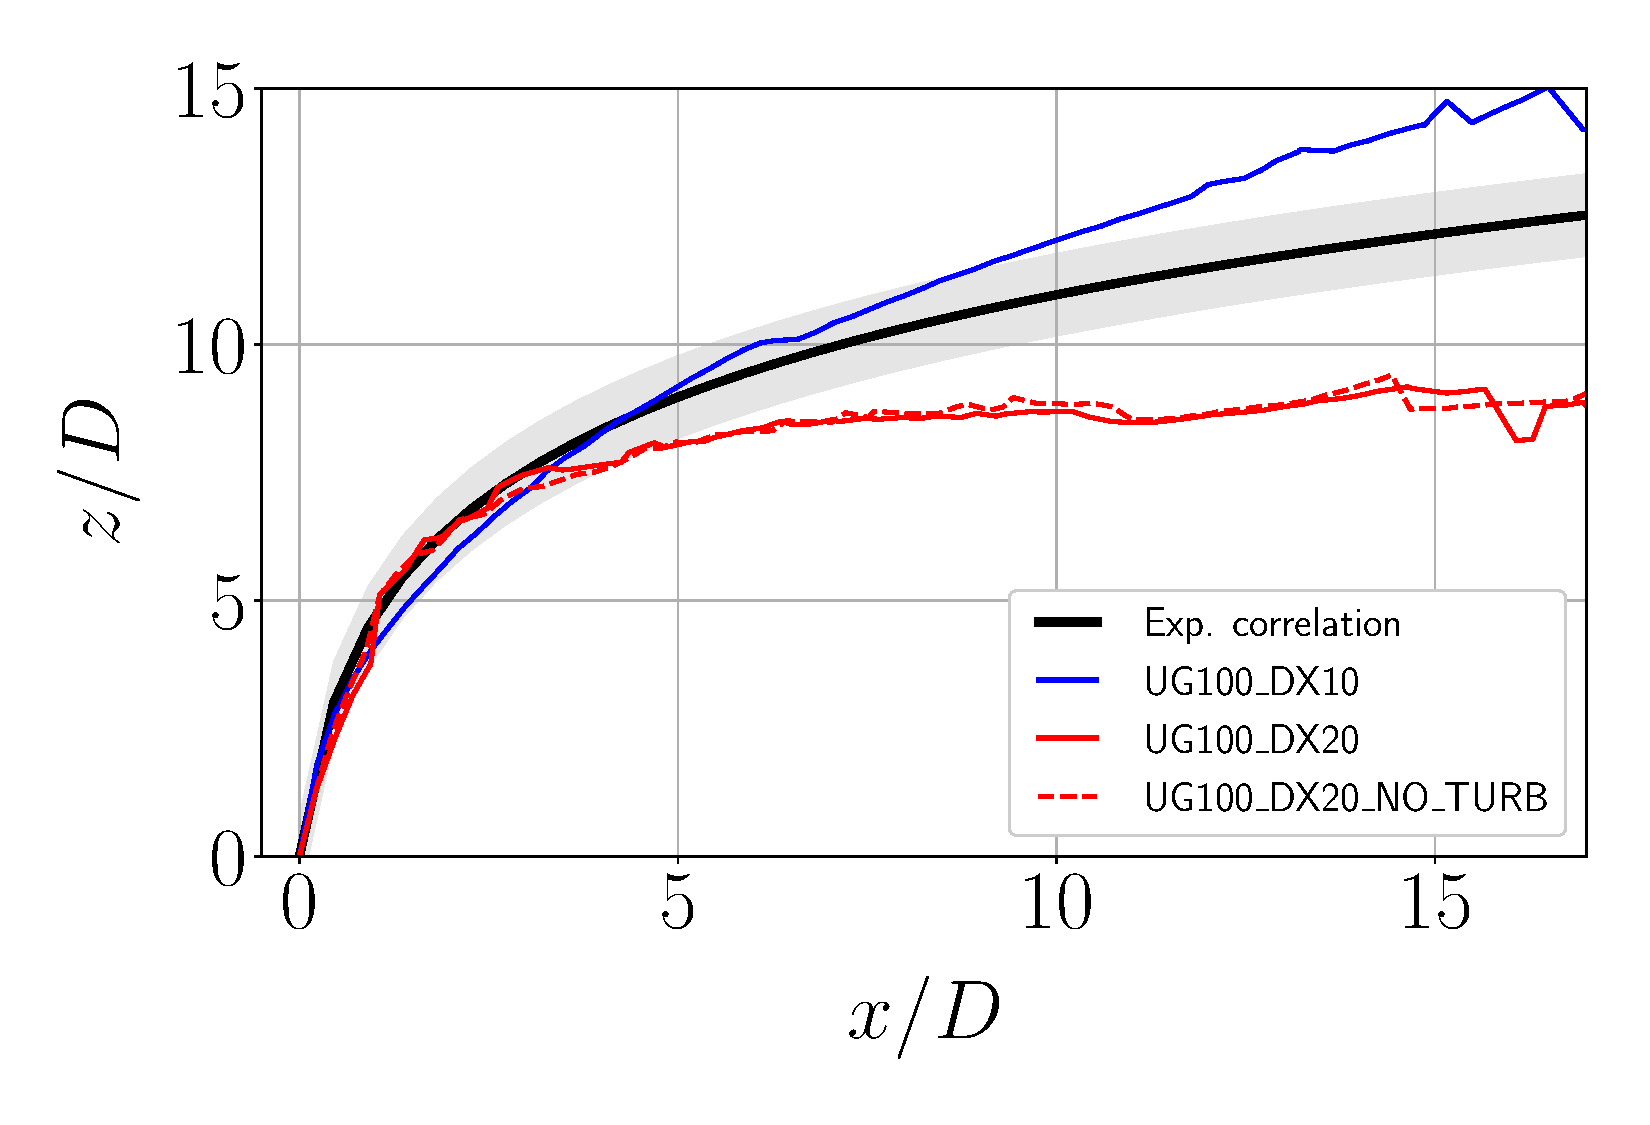
\includegraphics[scale=0.15]{./part2_developments/figures_ch5_resolved_JICF/results_trajectories/methods_expe_validation_trajectories_q6uG100.pdf}
   \caption{Low $We$}
   %\label{}
\end{subfigure}
\caption{Trajectories obtained with methods MEAN\_GRAD}
\label{fig:JICF_trajectories_validation}
\end{figure}

Slip velocity:

\begin{equation}
\overline{\textbf{u}}_{\mathrm{sl}} = \overline{\textbf{u}}_l - \overline{\textbf{u}}_g
\end{equation}


\section{Direct measurement of liquid flow rates}

Liquid fluxes have been measured in the resolved simulations at the planes shown in Figure \ref{fig:jicf_interior_boundaries_surface_measurements}. In the coarse simulations done with a mesh resolution of $\Delta x_\mathrm{min} = 20 \mu m$, fluxes have been obtained in all planes shown in the sketch. For the fine simulations, results were collected up to x = 10 mm since the liquid was removed shortly afterwards.

\subsection{Obtention of total flow rate}

The time evolution of flow rates for case UG100\_DX20 is shown in Figure \ref{fig:IB_liquid_flow_rate_inst_evolution_UG100_DX20} for both crossflow and filming planes. For the crossflow planes, the 

%\begin{figure}[h!]
%\centering
%\includegraphics[scale=0.6]{./part2_developments/figures_ch5_resolved_JICF/flow_rates_ibs/uG100_dx20_QL_isox_time_evol.eps}
%\caption{Liquid flow rate evolution with time in the}
%\label{fig:graphite_cp}
%\end{figure}

\begin{figure}[ht]
\centering
\begin{subfigure}[b]{0.45\textwidth}
	\centering
   \includegraphics[scale=0.15]{./part2_developments/figures_ch5_resolved_JICF/flow_rates_ibs/uG100_dx20_QL_isox_time_evol.eps}
   %\caption{}
   %\label{} 
\end{subfigure}
\begin{subfigure}[b]{0.45\textwidth}
	\centering
   \includegraphics[scale=0.15]{./part2_developments/figures_ch5_resolved_JICF/flow_rates_ibs/uG100_dx20_QL_filming_time_evol.eps}
   %\caption{}
   %\label{}
\end{subfigure}
\caption{Time evolution of instantaneous liquid flow rates for case UG100\_DX20. \textbf{Left}: planes normal to crossflow. \textbf{Right}: filming planes.}
\label{fig:IB_liquid_flow_rate_inst_evolution_UG100_DX20}
\end{figure}

\newpage

\begin{figure}[ht]
\centering
\begin{subfigure}[b]{0.45\textwidth}
	\centering
   \includegraphics[scale=0.17]{./part2_developments/figures_ch5_resolved_JICF/flow_rates_ibs/uG100_dx20_QL_isox_mean_time_convergence.eps}
   \caption{Mean $Q_l$ in crossflow planes}
   %\label{} 
\end{subfigure}
\hfill
\begin{subfigure}[b]{0.45\textwidth}
	\centering
   \includegraphics[scale=0.17]{./part2_developments/figures_ch5_resolved_JICF/flow_rates_ibs/uG100_dx20_QL_isox_RMS_time_convergence.eps}
   \caption{RMS $Q_l$ in crossflow planes}
   %\label{}
\end{subfigure}
\vskip\baselineskip
\begin{subfigure}[b]{0.45\textwidth}
	\centering
   \includegraphics[scale=0.17]{./part2_developments/figures_ch5_resolved_JICF/flow_rates_ibs/uG100_dx20_QL_filming_mean_time_convergence.eps}
   \caption{Mean $Q_l$ in filming planes}
   %\label{} 
\end{subfigure}
\hfill
\begin{subfigure}[b]{0.45\textwidth}
	\centering
   \includegraphics[scale=0.17]{./part2_developments/figures_ch5_resolved_JICF/flow_rates_ibs/uG100_dx20_QL_filming_RMS_time_convergence.eps}
   \caption{RMS $Q_l$ in filming planes}
   %\label{}
\end{subfigure}
\caption{Time evolution of mean and RMS liquid flow rates for case UG100\_DX20.}
\label{fig:IB_liquid_flow_rate_mean_RMS_evolution_UG100_DX20}
\end{figure}

\newpage

\begin{figure}[ht]
\centering
\begin{subfigure}[b]{0.45\textwidth}
	\centering
   \includegraphics[scale=0.10]{./part2_developments/figures_ch5_resolved_JICF/flow_rates_ibs/uG100_dx20_QL_isox_bar_plot.eps}
   \caption{Case UG100\_DX20: crossflow planes}
   %\label{} 
\end{subfigure}
\hfill
\begin{subfigure}[b]{0.45\textwidth}
	\centering
   \includegraphics[scale=0.10]{./part2_developments/figures_ch5_resolved_JICF/flow_rates_ibs/uG100_dx20_QL_filming_bar_plot.eps}
   \caption{Case UG100\_DX20: filming planes}
   %\label{}
\end{subfigure}
\vskip\baselineskip
\begin{subfigure}[b]{0.45\textwidth}
	\centering
   \includegraphics[scale=0.10]{./part2_developments/figures_ch5_resolved_JICF/flow_rates_ibs/uG100_dx10_QL_isox_bar_plot.eps}
   \caption{Case UG100\_DX10: crossflow planes}
   %\label{} 
\end{subfigure}
\hfill
\begin{subfigure}[b]{0.45\textwidth}
	\centering
   \includegraphics[scale=0.10]{./part2_developments/figures_ch5_resolved_JICF/flow_rates_ibs/uG100_dx10_QL_filming_bar_plot.eps}
   \caption{Case UG100\_DX10: filming planes}
   %\label{}
\end{subfigure}

\vskip\baselineskip

\begin{subfigure}[b]{0.45\textwidth}
	\centering
   \includegraphics[scale=0.10]{./part2_developments/figures_ch5_resolved_JICF/flow_rates_ibs/uG75_dx20_QL_isox_bar_plot.eps}
   \caption{Case UG75\_DX20: crossflow planes}
   %\label{} 
\end{subfigure}
\hfill
\begin{subfigure}[b]{0.45\textwidth}
	\centering
   \includegraphics[scale=0.10]{./part2_developments/figures_ch5_resolved_JICF/flow_rates_ibs/uG75_dx20_QL_filming_bar_plot.eps}
   \caption{Case UG75\_DX20: filming planes}
   %\label{}
\end{subfigure}
\vskip\baselineskip
\begin{subfigure}[b]{0.45\textwidth}
	\centering
   \includegraphics[scale=0.10]{./part2_developments/figures_ch5_resolved_JICF/flow_rates_ibs/uG75_dx10_QL_isox_bar_plot.eps}
   \caption{Case UG75\_DX10: crossflow planes}
   %\label{} 
\end{subfigure}
\hfill
\begin{subfigure}[b]{0.45\textwidth}
	\centering
   \includegraphics[scale=0.10]{./part2_developments/figures_ch5_resolved_JICF/flow_rates_ibs/uG75_dx10_QL_filming_bar_plot.eps}
   \caption{Case UG75\_DX10: filming planes}
   %\label{}
\end{subfigure}
\caption[Mean flow rates (bars) and RMS (lines) obtained with interior boundaries for each simulation performed]{Mean flow rates (bars) and RMS (lines) obtained with interior boundaries for each simulation performed. }
\label{fig:JICF_ibs_flow_rates_bars_plots}
\end{figure}









\subsection{Spatial distribution of flow rates in crossflow planes}




\newpage

\subsection{Mass conservation in ACLS}

%\subsubsection{Sampling procedure for droplets}

\newpage

\section{Spray characterization}

The number of droplets accumulated in each sampling plane for all the simulations performed in shown in Figure \ref{tab:jicf_Ndr_accumulated}.

\begin{table}[!h]
\centering
\caption{Number of droplets accumulated in JICF simulations}
\begin{tabular}{rcccc}
\thickhline
\textbf{Case} & $x = 5$ mm & $x = 10$ mm & $x = 15$ mm  & $x = 20$ mm \\
\thickhline 
UG75\_DX10  & 14233 & 20677 & - & - \\
UG75\_DX20  &  6882 & 12224 & 12077 & 9440 \\
UG100\_DX10 & 16442 & 11087 & - & -\\
UG100\_DX20 & 21824 & 17793 & 9476 & 11041 \\
\thickhline
\end{tabular}
\label{tab:jicf_Ndr_accumulated}
\end{table}

For the histograms, we can see 2013 Vie.


\subsection{Deformation variation with axial distance}

\subsection{Granulometry}

Sprays generated by atomization processes can be characterized by means of distributions. A given spray where the sizes of the droplets are known can be studied by representing distributions which express the probability of finding a droplet diameter or volume in that spray. Size distributions are usually representing by the notation $f_0 \left( D \right)$, while volume distributions are denoted by $f_3 \left( D \right)$. Two types of distributions are possible: discrete (histograms) or continuous. In the former, the spectrum of droplets size is divided into several range of droplets named bins or classes, and the number of droplets comprised within each class each counted. Histograms are the usual way of representing the granulometry when the size of droplets is directly available, such as in most experimental campaings and computational studies resolving atomization. Continuous distributions, however, are often used to fit discrete distributions obtained experimentally and are used for making simplified models for spray injection in lagrangian simulations, since they can represent the spray by functions depending on few parameters. Examples of function widely used in sprays are the lognormal, Rosin-Rammler and Nukiyama-Tanasama distributions \citepColor[lefebvre_atomization_2017]. 

Since in the resolved simulations performed in the work the size and volume of droplets are known (formally, the volume is known but the size is estimated with Eq. \ref{eq:ch4_r_equivalent_calculation}), probability histograms can be plotted. Figure \ref{fig:JICF_histograms_ug100_dx20} shows size (left) and volume (right) histograms for the sprays obtained from the case UG100\_DX20. The number of classes has been calculated according to Rice's rule, which estimates this value as $N_\mathrm{bins} = \sqrt[3]{2 N_\mathrm{dr}}$ \citepColor[terrel_oversmoothed_1985].




Size distributions can be represented by means of histograms relating the probability of finding a droplet with a given size with respect to the diameter, $f_0 \left( D \right)$.



In \citeColor[lefebvre_atomization_2017] ...



\textbf{Log-normal distribution}. This distribution function is more representative of certain types of atomizers, such as the spray produced by the jet in crossflow. In contrast to the normal distribution, the log-normal distribution takes the logarithm of the particle diameter as a variable. It is given by the following expression, where $\overline{D}_{ng}$ is the geometric mean size of the logarithmic droplet size and $s_g$ is the geometric standard deviation:

\begin{equation}
 f_0 \left( D \right) = \frac{d N}{d D} =  \frac{1}{D  \sqrt{2 \pi \ln \left( s_g \right)^2}} \exp \left[ - \frac{1}{2 } \left( \frac{\ln D - \ln \overline{D}_{ng}}{\ln s_g}   \right)^2 \right]
\end{equation}
%
\begin{equation}
\overline{D}_{ng} = \exp \left(  \frac{\sum_i \ln D_i }{N_\mathrm{droplets}} \right) 
\end{equation}

\begin{equation}
s_g = \exp \sqrt{  \frac{\sum_i \ln \left( D_i / \overline{D}_{ng} \right) ^2 }{N_\mathrm{droplets}} }
\end{equation}




\begin{figure}[ht]
\centering
\begin{subfigure}[b]{0.45\textwidth}
	\centering
   \includegraphics[scale=0.30]{./part2_developments/figures_ch5_resolved_JICF/spray_distributions/uG100_dx20_x05_number_histogram.eps}
   \caption{x = 5 mm, number histogram}
   %\label{} 
\end{subfigure}
\hfill
\begin{subfigure}[b]{0.45\textwidth}
	\centering
   \includegraphics[scale=0.30]{./part2_developments/figures_ch5_resolved_JICF/spray_distributions/uG100_dx20_x05_volume_histogram.eps}
   \caption{x = 5 mm, volume histogram}
   %\label{}
\end{subfigure}
\vskip\baselineskip
\begin{subfigure}[b]{0.45\textwidth}
	\centering
   \includegraphics[scale=0.30]{./part2_developments/figures_ch5_resolved_JICF/spray_distributions/uG100_dx20_x10_number_histogram.eps}
   \caption{x = 10 mm, number histogram}
   %\label{} 
\end{subfigure}
\hfill
\begin{subfigure}[b]{0.45\textwidth}
	\centering
   \includegraphics[scale=0.30]{./part2_developments/figures_ch5_resolved_JICF/spray_distributions/uG100_dx20_x10_volume_histogram.eps}
   \caption{x = 10 mm, volume histogram}
   %\label{}
\end{subfigure}
\vskip\baselineskip
\begin{subfigure}[b]{0.45\textwidth}
	\centering
   \includegraphics[scale=0.30]{./part2_developments/figures_ch5_resolved_JICF/spray_distributions/uG100_dx20_x15_number_histogram.eps}
   \caption{x = 15 mm, number histogram}
   %\label{} 
\end{subfigure}
\hfill
\begin{subfigure}[b]{0.45\textwidth}
	\centering
   \includegraphics[scale=0.30]{./part2_developments/figures_ch5_resolved_JICF/spray_distributions/uG100_dx20_x15_volume_histogram.eps}
   \caption{x = 15 mm, volume histogram}
   %\label{}
\end{subfigure}
\vskip\baselineskip
\begin{subfigure}[b]{0.45\textwidth}
	\centering
   \includegraphics[scale=0.30]{./part2_developments/figures_ch5_resolved_JICF/spray_distributions/uG100_dx20_x20_number_histogram.eps}
   \caption{x = 20 mm, number histogram}
   %\label{} 
\end{subfigure}
\hfill
\begin{subfigure}[b]{0.45\textwidth}
	\centering
   \includegraphics[scale=0.30]{./part2_developments/figures_ch5_resolved_JICF/spray_distributions/uG100_dx20_x20_volume_histogram.eps}
   \caption{x = 20 mm, volume histogram}
   %\label{}
\end{subfigure}
\caption{Histograms and lognormal fits for sampling planes in case UG100\_DX20}
\label{fig:JICF_histograms_ug100_dx20}
\end{figure}


\begin{figure}[ht]
\centering
   \includegraphics[scale=0.30]{./part2_developments/figures_ch5_resolved_JICF/SMD_values.eps}
   \caption{Evolution of SMD with axial distance for each simulation}
   \label{}
\end{figure}

\subsection{Definition of characteristic times}

Several characteristic times can be defined in a jet in crossflow:

\begin{itemize}

	\item Characteristic time of ligaments passage at given planes, $t_\mathrm{pas}$
	
	\item Characteristic time related to the frequency of the instabilities causing column breakup, $t_\mathrm{ins}$
	
	\item Physical definition according to ...

\end{itemize}


\begin{equation}
t^* = \frac{t}{\tau_\mathrm{dr}}
\end{equation}

\section{Dense core characterization}
\label{subsec:ch5_dense_core_in_ACLS_simus}

Resolved simulations are characterized by the presence of the dense core, whose presence perturbs the incoming air and creates turbulence downstream the injector. To illustrate this disturbance, the instantaneous axial fluctuations $u'$ and the jet interface are plotted in the middle plane y = 0 in Figure \ref{fig:results_dense_core_modeling_up_field} left. As shown, the jet presence

\begin{figure}[ht]
\centering
\includeinkscape[inkscapelatex=false,scale=0.75]{./part2_developments/figures_ch5_resolved_JICF/results_dense_core_modeling/up_field_instantaneous}
\caption[Perturbation effect of the liquid dense core in the gaseous field.]{Instantaneous $u'$ field in a JICF simulation from case UG100\_DX20. The black contours indicate the lines with zero instantaneous fluctuation $u' = 0$, while the white contours denote the location of the interface at the plane.}
\label{fig:results_dense_core_modeling_up_field}
\end{figure}



$\S$\ref{sec:ch4_dense_core_modelling}.

Patil correlations:

\begin{equation}
\frac{\overline{z_b}}{d_\mathrm{inj}} = 1.48 q^{0.3} We_g^{0.1} ~~~~; \frac{\overline{x_b}}{d_\mathrm{inj}} = 8.6 q^{-0.4}
\end{equation}

\section{Frequential analysis}

A spectral analysis is performed to obtain the characteristic breakup frequencies. There are several ways to obtain the desired frequencies:

\begin{itemize}

	\item Use Proper Orthogonal Decomposition (POD) technique (2018 Prakash, Mukundan). This is out of the scope of this work.
	
	\item Get evolution of breakup point with time: $x_b \left( t \right)$, $z_b \left( t \right)$, then get the frequency spectrum  (2010 Wang, 2018 Prakash). Not sure we can do this with our available data, so not envisageable now.
	
	\item Locate probes along liquid column, get liquid presence rate with time. This is the one !!

\end{itemize}

\section{Computational performances}
\label{subsec:ch5_computational_performances}

%\subsection{Feeding the models (??)}
%Find a more attractive name

\section{Learning injectors}



\subsection{Spatial discretization of sprays}

\clearpage

\subsection{Case UG75\_DX10}



%%%%%%%%%%%%%%%% UG75_DX10, x = 5 mm


\begin{figure}[h!]
\flushleft
\begin{subfigure}[b]{0.22\textwidth}
	\centering
   \includegraphics[scale=0.17]{./part2_developments/figures_ch5_resolved_JICF/injectors_SLI/uG75_dx10_x05_SMD_map.eps}
   %\caption{Case UG100\_DX20: crossflow planes}
   %\label{} 
\end{subfigure}
   \hspace{0.17in}
\begin{subfigure}[b]{0.22\textwidth}
	\centering
   \includegraphics[scale=0.17]{./part2_developments/figures_ch5_resolved_JICF/injectors_SLI/uG75_dx10_x05_ux_mean_map.eps}
   %\caption{Case UG100\_DX20: filming planes}
   %\label{}
\end{subfigure}
   \hspace{0.17in}
\begin{subfigure}[b]{0.22\textwidth}
	\centering
   \includegraphics[scale=0.17]{./part2_developments/figures_ch5_resolved_JICF/injectors_SLI/uG75_dx10_x05_uy_mean_map.eps}
   %\caption{Case UG100\_DX10: crossflow planes}
   %\label{} 
\end{subfigure}
   \hspace{0.17in}
\begin{subfigure}[b]{0.22\textwidth}
	\centering
   \includegraphics[scale=0.17]{./part2_developments/figures_ch5_resolved_JICF/injectors_SLI/uG75_dx10_x05_uz_mean_map.eps}
   %\caption{Case UG100\_DX10: filming planes}
   %\label{}
\end{subfigure}

\vskip\baselineskip

\begin{subfigure}[b]{0.22\textwidth}
	\centering
   \includegraphics[scale=0.17]{./part2_developments/figures_ch5_resolved_JICF/injectors_SLI/uG75_dx10_x05_volume_flux_map.eps}
   %\caption{Case UG100\_DX20: crossflow planes}
   %\label{} 
\end{subfigure}
   \hspace{0.17in}
\begin{subfigure}[b]{0.22\textwidth}
	\centering
   \includegraphics[scale=0.17]{./part2_developments/figures_ch5_resolved_JICF/injectors_SLI/uG75_dx10_x05_ux_rms_map.eps}
   %\caption{Case UG100\_DX20: filming planes}
   %\label{}
\end{subfigure}
   \hspace{0.17in}
\begin{subfigure}[b]{0.22\textwidth}
	\centering
   \includegraphics[scale=0.17]{./part2_developments/figures_ch5_resolved_JICF/injectors_SLI/uG75_dx10_x05_uy_rms_map.eps}
   %\caption{Case UG100\_DX10: crossflow planes}
   %\label{} 
\end{subfigure}
   \hspace{0.17in}
\begin{subfigure}[b]{0.22\textwidth}
	\centering
   \includegraphics[scale=0.17]{./part2_developments/figures_ch5_resolved_JICF/injectors_SLI/uG75_dx10_x05_uz_rms_map.eps}
   %\caption{Case UG100\_DX10: filming planes}
   %\label{}
\end{subfigure}
\caption{Spray states at x = 5 mm for case UG75\_DX10}
\label{fig:injectors_sli_uG75_dx10_x05}
\end{figure}


%%%%%%%%%%%%%%%% UG75_DX10, x = 10 mm


\begin{figure}[h!]
\flushleft
\begin{subfigure}[b]{0.22\textwidth}
	\centering
   \includegraphics[scale=0.17]{./part2_developments/figures_ch5_resolved_JICF/injectors_SLI/uG75_dx10_x10_SMD_map.eps}
   %\caption{Case UG100\_DX20: crossflow planes}
   %\label{} 
\end{subfigure}
   \hspace{0.17in}
\begin{subfigure}[b]{0.22\textwidth}
	\centering
   \includegraphics[scale=0.17]{./part2_developments/figures_ch5_resolved_JICF/injectors_SLI/uG75_dx10_x10_ux_mean_map.eps}
   %\caption{Case UG100\_DX20: filming planes}
   %\label{}
\end{subfigure}
   \hspace{0.17in}
\begin{subfigure}[b]{0.22\textwidth}
	\centering
   \includegraphics[scale=0.17]{./part2_developments/figures_ch5_resolved_JICF/injectors_SLI/uG75_dx10_x10_uy_mean_map.eps}
   %\caption{Case UG100\_DX10: crossflow planes}
   %\label{} 
\end{subfigure}
   \hspace{0.17in}
\begin{subfigure}[b]{0.22\textwidth}
	\centering
   \includegraphics[scale=0.17]{./part2_developments/figures_ch5_resolved_JICF/injectors_SLI/uG75_dx10_x10_uz_mean_map.eps}
   %\caption{Case UG100\_DX10: filming planes}
   %\label{}
\end{subfigure}

\vskip\baselineskip

\begin{subfigure}[b]{0.22\textwidth}
	\centering
   \includegraphics[scale=0.17]{./part2_developments/figures_ch5_resolved_JICF/injectors_SLI/uG75_dx10_x10_volume_flux_map.eps}
   %\caption{Case UG100\_DX20: crossflow planes}
   %\label{} 
\end{subfigure}
   \hspace{0.17in}
\begin{subfigure}[b]{0.22\textwidth}
	\centering
   \includegraphics[scale=0.17]{./part2_developments/figures_ch5_resolved_JICF/injectors_SLI/uG75_dx10_x10_ux_rms_map.eps}
   %\caption{Case UG100\_DX20: filming planes}
   %\label{}
\end{subfigure}
   \hspace{0.17in}
\begin{subfigure}[b]{0.22\textwidth}
	\centering
   \includegraphics[scale=0.17]{./part2_developments/figures_ch5_resolved_JICF/injectors_SLI/uG75_dx10_x10_uy_rms_map.eps}
   %\caption{Case UG100\_DX10: crossflow planes}
   %\label{} 
\end{subfigure}
   \hspace{0.17in}
\begin{subfigure}[b]{0.22\textwidth}
	\centering
   \includegraphics[scale=0.17]{./part2_developments/figures_ch5_resolved_JICF/injectors_SLI/uG75_dx10_x10_uz_rms_map.eps}
   %\caption{Case UG100\_DX10: filming planes}
   %\label{}
\end{subfigure}
\caption{Spray states at x = 10 mm for case UG75\_DX10}
\label{fig:injectors_sli_uG75_dx10_x10}
\end{figure}


\clearpage

\subsection{Case UG75\_DX20}



%%%%%%%%%%%%%%%% UG75_DX20, x = 5 mm


\begin{figure}[h!]
\flushleft
\begin{subfigure}[b]{0.22\textwidth}
	\centering
   \includegraphics[scale=0.17]{./part2_developments/figures_ch5_resolved_JICF/injectors_SLI/uG75_dx20_x05_SMD_map.eps}
   %\caption{Case UG100\_DX20: crossflow planes}
   %\label{} 
\end{subfigure}
   \hspace{0.17in}
\begin{subfigure}[b]{0.22\textwidth}
	\centering
   \includegraphics[scale=0.17]{./part2_developments/figures_ch5_resolved_JICF/injectors_SLI/uG75_dx20_x05_ux_mean_map.eps}
   %\caption{Case UG100\_DX20: filming planes}
   %\label{}
\end{subfigure}
   \hspace{0.17in}
\begin{subfigure}[b]{0.22\textwidth}
	\centering
   \includegraphics[scale=0.17]{./part2_developments/figures_ch5_resolved_JICF/injectors_SLI/uG75_dx20_x05_uy_mean_map.eps}
   %\caption{Case UG100\_DX10: crossflow planes}
   %\label{} 
\end{subfigure}
   \hspace{0.17in}
\begin{subfigure}[b]{0.22\textwidth}
	\centering
   \includegraphics[scale=0.17]{./part2_developments/figures_ch5_resolved_JICF/injectors_SLI/uG75_dx20_x05_uz_mean_map.eps}
   %\caption{Case UG100\_DX10: filming planes}
   %\label{}
\end{subfigure}

\vskip\baselineskip

\begin{subfigure}[b]{0.22\textwidth}
	\centering
   \includegraphics[scale=0.17]{./part2_developments/figures_ch5_resolved_JICF/injectors_SLI/uG75_dx20_x05_volume_flux_map.eps}
   %\caption{Case UG100\_DX20: crossflow planes}
   %\label{} 
\end{subfigure}
   \hspace{0.17in}
\begin{subfigure}[b]{0.22\textwidth}
	\centering
   \includegraphics[scale=0.17]{./part2_developments/figures_ch5_resolved_JICF/injectors_SLI/uG75_dx20_x05_ux_rms_map.eps}
   %\caption{Case UG100\_DX20: filming planes}
   %\label{}
\end{subfigure}
   \hspace{0.17in}
\begin{subfigure}[b]{0.22\textwidth}
	\centering
   \includegraphics[scale=0.17]{./part2_developments/figures_ch5_resolved_JICF/injectors_SLI/uG75_dx20_x05_uy_rms_map.eps}
   %\caption{Case UG100\_DX10: crossflow planes}
   %\label{} 
\end{subfigure}
   \hspace{0.17in}
\begin{subfigure}[b]{0.22\textwidth}
	\centering
   \includegraphics[scale=0.17]{./part2_developments/figures_ch5_resolved_JICF/injectors_SLI/uG75_dx20_x05_uz_rms_map.eps}
   %\caption{Case UG100\_DX10: filming planes}
   %\label{}
\end{subfigure}
\caption{Spray states at x = 5 mm for case UG75\_DX20}
\label{fig:injectors_sli_uG75_dx20_x05}
\end{figure}


%%%%%%%%%%%%%%%% UG75_DX10, x = 10 mm


\begin{figure}[h!]
\flushleft
\begin{subfigure}[b]{0.22\textwidth}
	\centering
   \includegraphics[scale=0.17]{./part2_developments/figures_ch5_resolved_JICF/injectors_SLI/uG75_dx20_x10_SMD_map.eps}
   %\caption{Case UG100\_DX20: crossflow planes}
   %\label{} 
\end{subfigure}
   \hspace{0.17in}
\begin{subfigure}[b]{0.22\textwidth}
	\centering
   \includegraphics[scale=0.17]{./part2_developments/figures_ch5_resolved_JICF/injectors_SLI/uG75_dx20_x10_ux_mean_map.eps}
   %\caption{Case UG100\_DX20: filming planes}
   %\label{}
\end{subfigure}
   \hspace{0.17in}
\begin{subfigure}[b]{0.22\textwidth}
	\centering
   \includegraphics[scale=0.17]{./part2_developments/figures_ch5_resolved_JICF/injectors_SLI/uG75_dx20_x10_uy_mean_map.eps}
   %\caption{Case UG100\_DX10: crossflow planes}
   %\label{} 
\end{subfigure}
   \hspace{0.17in}
\begin{subfigure}[b]{0.22\textwidth}
	\centering
   \includegraphics[scale=0.17]{./part2_developments/figures_ch5_resolved_JICF/injectors_SLI/uG75_dx20_x10_uz_mean_map.eps}
   %\caption{Case UG100\_DX10: filming planes}
   %\label{}
\end{subfigure}

\vskip\baselineskip

\begin{subfigure}[b]{0.22\textwidth}
	\centering
   \includegraphics[scale=0.17]{./part2_developments/figures_ch5_resolved_JICF/injectors_SLI/uG75_dx20_x10_volume_flux_map.eps}
   %\caption{Case UG100\_DX20: crossflow planes}
   %\label{} 
\end{subfigure}
   \hspace{0.17in}
\begin{subfigure}[b]{0.22\textwidth}
	\centering
   \includegraphics[scale=0.17]{./part2_developments/figures_ch5_resolved_JICF/injectors_SLI/uG75_dx20_x10_ux_rms_map.eps}
   %\caption{Case UG100\_DX20: filming planes}
   %\label{}
\end{subfigure}
   \hspace{0.17in}
\begin{subfigure}[b]{0.22\textwidth}
	\centering
   \includegraphics[scale=0.17]{./part2_developments/figures_ch5_resolved_JICF/injectors_SLI/uG75_dx20_x10_uy_rms_map.eps}
   %\caption{Case UG100\_DX10: crossflow planes}
   %\label{} 
\end{subfigure}
   \hspace{0.17in}
\begin{subfigure}[b]{0.22\textwidth}
	\centering
   \includegraphics[scale=0.17]{./part2_developments/figures_ch5_resolved_JICF/injectors_SLI/uG75_dx20_x10_uz_rms_map.eps}
   %\caption{Case UG100\_DX10: filming planes}
   %\label{}
\end{subfigure}
\caption{Spray states at x = 10 mm for case UG75\_DX20}
\label{fig:injectors_sli_uG75_dx20_x10}
\end{figure}


%%%%%%%%%%%%%%%% UG75_DX10, x = 15 mm


\begin{figure}[h!]
\flushleft
\begin{subfigure}[b]{0.22\textwidth}
	\centering
   \includegraphics[scale=0.17]{./part2_developments/figures_ch5_resolved_JICF/injectors_SLI/uG75_dx20_x15_SMD_map.eps}
   %\caption{Case UG100\_DX20: crossflow planes}
   %\label{} 
\end{subfigure}
   \hspace{0.17in}
\begin{subfigure}[b]{0.22\textwidth}
	\centering
   \includegraphics[scale=0.17]{./part2_developments/figures_ch5_resolved_JICF/injectors_SLI/uG75_dx20_x15_ux_mean_map.eps}
   %\caption{Case UG100\_DX20: filming planes}
   %\label{}
\end{subfigure}
   \hspace{0.17in}
\begin{subfigure}[b]{0.22\textwidth}
	\centering
   \includegraphics[scale=0.17]{./part2_developments/figures_ch5_resolved_JICF/injectors_SLI/uG75_dx20_x15_uy_mean_map.eps}
   %\caption{Case UG100\_DX10: crossflow planes}
   %\label{} 
\end{subfigure}
   \hspace{0.17in}
\begin{subfigure}[b]{0.22\textwidth}
	\centering
   \includegraphics[scale=0.17]{./part2_developments/figures_ch5_resolved_JICF/injectors_SLI/uG75_dx20_x15_uz_mean_map.eps}
   %\caption{Case UG100\_DX10: filming planes}
   %\label{}
\end{subfigure}

\vskip\baselineskip

\begin{subfigure}[b]{0.22\textwidth}
	\centering
   \includegraphics[scale=0.17]{./part2_developments/figures_ch5_resolved_JICF/injectors_SLI/uG75_dx20_x15_volume_flux_map.eps}
   %\caption{Case UG100\_DX20: crossflow planes}
   %\label{} 
\end{subfigure}
   \hspace{0.17in}
\begin{subfigure}[b]{0.22\textwidth}
	\centering
   \includegraphics[scale=0.17]{./part2_developments/figures_ch5_resolved_JICF/injectors_SLI/uG75_dx20_x15_ux_rms_map.eps}
   %\caption{Case UG100\_DX20: filming planes}
   %\label{}
\end{subfigure}
   \hspace{0.17in}
\begin{subfigure}[b]{0.22\textwidth}
	\centering
   \includegraphics[scale=0.17]{./part2_developments/figures_ch5_resolved_JICF/injectors_SLI/uG75_dx20_x15_uy_rms_map.eps}
   %\caption{Case UG100\_DX10: crossflow planes}
   %\label{} 
\end{subfigure}
   \hspace{0.17in}
\begin{subfigure}[b]{0.22\textwidth}
	\centering
   \includegraphics[scale=0.17]{./part2_developments/figures_ch5_resolved_JICF/injectors_SLI/uG75_dx20_x15_uz_rms_map.eps}
   %\caption{Case UG100\_DX10: filming planes}
   %\label{}
\end{subfigure}
\caption{Spray states at x = 15 mm for case UG75\_DX20}
\label{fig:injectors_sli_uG75_dx20_x15}
\end{figure}


\clearpage

\subsection{Case UG100\_DX10}



%%%%%%%%%%%%%%%% UG100_DX10, x = 5 mm


\begin{figure}[h!]
\flushleft
\begin{subfigure}[b]{0.22\textwidth}
	\centering
   \includegraphics[scale=0.17]{./part2_developments/figures_ch5_resolved_JICF/injectors_SLI/uG100_dx10_x05_SMD_map.eps}
   %\caption{Case UG100\_DX20: crossflow planes}
   %\label{} 
\end{subfigure}
   \hspace{0.17in}
\begin{subfigure}[b]{0.22\textwidth}
	\centering
   \includegraphics[scale=0.17]{./part2_developments/figures_ch5_resolved_JICF/injectors_SLI/uG100_dx10_x05_ux_mean_map.eps}
   %\caption{Case UG100\_DX20: filming planes}
   %\label{}
\end{subfigure}
   \hspace{0.17in}
\begin{subfigure}[b]{0.22\textwidth}
	\centering
   \includegraphics[scale=0.17]{./part2_developments/figures_ch5_resolved_JICF/injectors_SLI/uG100_dx10_x05_uy_mean_map.eps}
   %\caption{Case UG100\_DX10: crossflow planes}
   %\label{} 
\end{subfigure}
   \hspace{0.17in}
\begin{subfigure}[b]{0.22\textwidth}
	\centering
   \includegraphics[scale=0.17]{./part2_developments/figures_ch5_resolved_JICF/injectors_SLI/uG100_dx10_x05_uz_mean_map.eps}
   %\caption{Case UG100\_DX10: filming planes}
   %\label{}
\end{subfigure}

\vskip\baselineskip

\begin{subfigure}[b]{0.22\textwidth}
	\centering
   \includegraphics[scale=0.17]{./part2_developments/figures_ch5_resolved_JICF/injectors_SLI/uG100_dx10_x05_volume_flux_map.eps}
   %\caption{Case UG100\_DX20: crossflow planes}
   %\label{} 
\end{subfigure}
   \hspace{0.17in}
\begin{subfigure}[b]{0.22\textwidth}
	\centering
   \includegraphics[scale=0.17]{./part2_developments/figures_ch5_resolved_JICF/injectors_SLI/uG100_dx10_x05_ux_rms_map.eps}
   %\caption{Case UG100\_DX20: filming planes}
   %\label{}
\end{subfigure}
   \hspace{0.17in}
\begin{subfigure}[b]{0.22\textwidth}
	\centering
   \includegraphics[scale=0.17]{./part2_developments/figures_ch5_resolved_JICF/injectors_SLI/uG100_dx10_x05_uy_rms_map.eps}
   %\caption{Case UG100\_DX10: crossflow planes}
   %\label{} 
\end{subfigure}
   \hspace{0.17in}
\begin{subfigure}[b]{0.22\textwidth}
	\centering
   \includegraphics[scale=0.17]{./part2_developments/figures_ch5_resolved_JICF/injectors_SLI/uG100_dx10_x05_uz_rms_map.eps}
   %\caption{Case UG100\_DX10: filming planes}
   %\label{}
\end{subfigure}
\caption{Spray states at x = 5 mm for case UG100\_DX10}
\label{fig:injectors_sli_uG100_dx10_x05}
\end{figure}


%%%%%%%%%%%%%%%% UG100_DX10, x = 10 mm


\begin{figure}[h!]
\flushleft
\begin{subfigure}[b]{0.22\textwidth}
	\centering
   \includegraphics[scale=0.17]{./part2_developments/figures_ch5_resolved_JICF/injectors_SLI/uG100_dx10_x10_SMD_map.eps}
   %\caption{Case UG100\_DX20: crossflow planes}
   %\label{} 
\end{subfigure}
   \hspace{0.17in}
\begin{subfigure}[b]{0.22\textwidth}
	\centering
   \includegraphics[scale=0.17]{./part2_developments/figures_ch5_resolved_JICF/injectors_SLI/uG100_dx10_x10_ux_mean_map.eps}
   %\caption{Case UG100\_DX20: filming planes}
   %\label{}
\end{subfigure}
   \hspace{0.17in}
\begin{subfigure}[b]{0.22\textwidth}
	\centering
   \includegraphics[scale=0.17]{./part2_developments/figures_ch5_resolved_JICF/injectors_SLI/uG100_dx10_x10_uy_mean_map.eps}
   %\caption{Case UG100\_DX10: crossflow planes}
   %\label{} 
\end{subfigure}
   \hspace{0.17in}
\begin{subfigure}[b]{0.22\textwidth}
	\centering
   \includegraphics[scale=0.17]{./part2_developments/figures_ch5_resolved_JICF/injectors_SLI/uG100_dx10_x10_uz_mean_map.eps}
   %\caption{Case UG100\_DX10: filming planes}
   %\label{}
\end{subfigure}

\vskip\baselineskip

\begin{subfigure}[b]{0.22\textwidth}
	\centering
   \includegraphics[scale=0.17]{./part2_developments/figures_ch5_resolved_JICF/injectors_SLI/uG100_dx10_x10_volume_flux_map.eps}
   %\caption{Case UG100\_DX20: crossflow planes}
   %\label{} 
\end{subfigure}
   \hspace{0.17in}
\begin{subfigure}[b]{0.22\textwidth}
	\centering
   \includegraphics[scale=0.17]{./part2_developments/figures_ch5_resolved_JICF/injectors_SLI/uG100_dx10_x10_ux_rms_map.eps}
   %\caption{Case UG100\_DX20: filming planes}
   %\label{}
\end{subfigure}
   \hspace{0.17in}
\begin{subfigure}[b]{0.22\textwidth}
	\centering
   \includegraphics[scale=0.17]{./part2_developments/figures_ch5_resolved_JICF/injectors_SLI/uG100_dx10_x10_uy_rms_map.eps}
   %\caption{Case UG100\_DX10: crossflow planes}
   %\label{} 
\end{subfigure}
   \hspace{0.17in}
\begin{subfigure}[b]{0.22\textwidth}
	\centering
   \includegraphics[scale=0.17]{./part2_developments/figures_ch5_resolved_JICF/injectors_SLI/uG100_dx10_x10_uz_rms_map.eps}
   %\caption{Case UG100\_DX10: filming planes}
   %\label{}
\end{subfigure}
\caption{Spray states at x = 10 mm for case UG100\_DX10}
\label{fig:injectors_sli_uG100_dx10_x10}
\end{figure}


\clearpage

\subsection{Case UG100\_DX20}



%%%%%%%%%%%%%%%% UG100_DX20, x = 5 mm


\begin{figure}[h!]
\flushleft
\begin{subfigure}[b]{0.22\textwidth}
	\centering
   \includegraphics[scale=0.17]{./part2_developments/figures_ch5_resolved_JICF/injectors_SLI/uG100_dx20_x05_SMD_map.eps}
   %\caption{Case UG100\_DX20: crossflow planes}
   %\label{} 
\end{subfigure}
   \hspace{0.17in}
\begin{subfigure}[b]{0.22\textwidth}
	\centering
   \includegraphics[scale=0.17]{./part2_developments/figures_ch5_resolved_JICF/injectors_SLI/uG100_dx20_x05_ux_mean_map.eps}
   %\caption{Case UG100\_DX20: filming planes}
   %\label{}
\end{subfigure}
   \hspace{0.17in}
\begin{subfigure}[b]{0.22\textwidth}
	\centering
   \includegraphics[scale=0.17]{./part2_developments/figures_ch5_resolved_JICF/injectors_SLI/uG100_dx20_x05_uy_mean_map.eps}
   %\caption{Case UG100\_DX10: crossflow planes}
   %\label{} 
\end{subfigure}
   \hspace{0.17in}
\begin{subfigure}[b]{0.22\textwidth}
	\centering
   \includegraphics[scale=0.17]{./part2_developments/figures_ch5_resolved_JICF/injectors_SLI/uG100_dx20_x05_uz_mean_map.eps}
   %\caption{Case UG100\_DX10: filming planes}
   %\label{}
\end{subfigure}

\vskip\baselineskip

\begin{subfigure}[b]{0.22\textwidth}
	\centering
   \includegraphics[scale=0.17]{./part2_developments/figures_ch5_resolved_JICF/injectors_SLI/uG100_dx20_x05_volume_flux_map.eps}
   %\caption{Case UG100\_DX20: crossflow planes}
   %\label{} 
\end{subfigure}
   \hspace{0.17in}
\begin{subfigure}[b]{0.22\textwidth}
	\centering
   \includegraphics[scale=0.17]{./part2_developments/figures_ch5_resolved_JICF/injectors_SLI/uG100_dx20_x05_ux_rms_map.eps}
   %\caption{Case UG100\_DX20: filming planes}
   %\label{}
\end{subfigure}
   \hspace{0.17in}
\begin{subfigure}[b]{0.22\textwidth}
	\centering
   \includegraphics[scale=0.17]{./part2_developments/figures_ch5_resolved_JICF/injectors_SLI/uG100_dx20_x05_uy_rms_map.eps}
   %\caption{Case UG100\_DX10: crossflow planes}
   %\label{} 
\end{subfigure}
   \hspace{0.17in}
\begin{subfigure}[b]{0.22\textwidth}
	\centering
   \includegraphics[scale=0.17]{./part2_developments/figures_ch5_resolved_JICF/injectors_SLI/uG100_dx20_x05_uz_rms_map.eps}
   %\caption{Case UG100\_DX10: filming planes}
   %\label{}
\end{subfigure}
\caption{Spray states at x = 5 mm for case UG100\_DX20}
\label{fig:injectors_sli_uG100_dx20_x05}
\end{figure}


%%%%%%%%%%%%%%%% UG100_DX10, x = 10 mm


\begin{figure}[h!]
\flushleft
\begin{subfigure}[b]{0.22\textwidth}
	\centering
   \includegraphics[scale=0.17]{./part2_developments/figures_ch5_resolved_JICF/injectors_SLI/uG100_dx20_x10_SMD_map.eps}
   %\caption{Case UG100\_DX20: crossflow planes}
   %\label{} 
\end{subfigure}
   \hspace{0.17in}
\begin{subfigure}[b]{0.22\textwidth}
	\centering
   \includegraphics[scale=0.17]{./part2_developments/figures_ch5_resolved_JICF/injectors_SLI/uG100_dx20_x10_ux_mean_map.eps}
   %\caption{Case UG100\_DX20: filming planes}
   %\label{}
\end{subfigure}
   \hspace{0.17in}
\begin{subfigure}[b]{0.22\textwidth}
	\centering
   \includegraphics[scale=0.17]{./part2_developments/figures_ch5_resolved_JICF/injectors_SLI/uG100_dx20_x10_uy_mean_map.eps}
   %\caption{Case UG100\_DX10: crossflow planes}
   %\label{} 
\end{subfigure}
   \hspace{0.17in}
\begin{subfigure}[b]{0.22\textwidth}
	\centering
   \includegraphics[scale=0.17]{./part2_developments/figures_ch5_resolved_JICF/injectors_SLI/uG100_dx20_x10_uz_mean_map.eps}
   %\caption{Case UG100\_DX10: filming planes}
   %\label{}
\end{subfigure}

\vskip\baselineskip

\begin{subfigure}[b]{0.22\textwidth}
	\centering
   \includegraphics[scale=0.17]{./part2_developments/figures_ch5_resolved_JICF/injectors_SLI/uG100_dx20_x10_volume_flux_map.eps}
   %\caption{Case UG100\_DX20: crossflow planes}
   %\label{} 
\end{subfigure}
   \hspace{0.17in}
\begin{subfigure}[b]{0.22\textwidth}
	\centering
   \includegraphics[scale=0.17]{./part2_developments/figures_ch5_resolved_JICF/injectors_SLI/uG100_dx20_x10_ux_rms_map.eps}
   %\caption{Case UG100\_DX20: filming planes}
   %\label{}
\end{subfigure}
   \hspace{0.17in}
\begin{subfigure}[b]{0.22\textwidth}
	\centering
   \includegraphics[scale=0.17]{./part2_developments/figures_ch5_resolved_JICF/injectors_SLI/uG100_dx20_x10_uy_rms_map.eps}
   %\caption{Case UG100\_DX10: crossflow planes}
   %\label{} 
\end{subfigure}
   \hspace{0.17in}
\begin{subfigure}[b]{0.22\textwidth}
	\centering
   \includegraphics[scale=0.17]{./part2_developments/figures_ch5_resolved_JICF/injectors_SLI/uG100_dx20_x10_uz_rms_map.eps}
   %\caption{Case UG100\_DX10: filming planes}
   %\label{}
\end{subfigure}
\caption{Spray states at x = 10 mm for case UG100\_DX20}
\label{fig:injectors_sli_uG100_dx20_x10}
\end{figure}


%%%%%%%%%%%%%%%% UG100_DX10, x = 15 mm


\begin{figure}[h!]
\flushleft
\begin{subfigure}[b]{0.22\textwidth}
	\centering
   \includegraphics[scale=0.17]{./part2_developments/figures_ch5_resolved_JICF/injectors_SLI/uG100_dx20_x15_SMD_map.eps}
   %\caption{Case UG100\_DX20: crossflow planes}
   %\label{} 
\end{subfigure}
   \hspace{0.17in}
\begin{subfigure}[b]{0.22\textwidth}
	\centering
   \includegraphics[scale=0.17]{./part2_developments/figures_ch5_resolved_JICF/injectors_SLI/uG100_dx20_x15_ux_mean_map.eps}
   %\caption{Case UG100\_DX20: filming planes}
   %\label{}
\end{subfigure}
   \hspace{0.17in}
\begin{subfigure}[b]{0.22\textwidth}
	\centering
   \includegraphics[scale=0.17]{./part2_developments/figures_ch5_resolved_JICF/injectors_SLI/uG100_dx20_x15_uy_mean_map.eps}
   %\caption{Case UG100\_DX10: crossflow planes}
   %\label{} 
\end{subfigure}
   \hspace{0.17in}
\begin{subfigure}[b]{0.22\textwidth}
	\centering
   \includegraphics[scale=0.17]{./part2_developments/figures_ch5_resolved_JICF/injectors_SLI/uG100_dx20_x15_uz_mean_map.eps}
   %\caption{Case UG100\_DX10: filming planes}
   %\label{}
\end{subfigure}

\vskip\baselineskip

\begin{subfigure}[b]{0.22\textwidth}
	\centering
   \includegraphics[scale=0.17]{./part2_developments/figures_ch5_resolved_JICF/injectors_SLI/uG100_dx20_x15_volume_flux_map.eps}
   %\caption{Case UG100\_DX20: crossflow planes}
   %\label{} 
\end{subfigure}
   \hspace{0.17in}
\begin{subfigure}[b]{0.22\textwidth}
	\centering
   \includegraphics[scale=0.17]{./part2_developments/figures_ch5_resolved_JICF/injectors_SLI/uG100_dx20_x15_ux_rms_map.eps}
   %\caption{Case UG100\_DX20: filming planes}
   %\label{}
\end{subfigure}
   \hspace{0.17in}
\begin{subfigure}[b]{0.22\textwidth}
	\centering
   \includegraphics[scale=0.17]{./part2_developments/figures_ch5_resolved_JICF/injectors_SLI/uG100_dx20_x15_uy_rms_map.eps}
   %\caption{Case UG100\_DX10: crossflow planes}
   %\label{} 
\end{subfigure}
   \hspace{0.17in}
\begin{subfigure}[b]{0.22\textwidth}
	\centering
   \includegraphics[scale=0.17]{./part2_developments/figures_ch5_resolved_JICF/injectors_SLI/uG100_dx20_x15_uz_rms_map.eps}
   %\caption{Case UG100\_DX10: filming planes}
   %\label{}
\end{subfigure}
\caption{Spray states at x = 15 mm for case UG100\_DX20}
\label{fig:injectors_sli_uG100_dx20_x15}
\end{figure}


\clearpage

\section{Conclusions}

